% Options for packages loaded elsewhere
\PassOptionsToPackage{unicode}{hyperref}
\PassOptionsToPackage{hyphens}{url}
\PassOptionsToPackage{space}{xeCJK}
\documentclass[
  a4paper,
]{article}
\usepackage{xcolor}
\usepackage[margin=24mm]{geometry}
\usepackage{amsmath,amssymb}
\setcounter{secnumdepth}{-\maxdimen} % remove section numbering
\usepackage{iftex}
\ifPDFTeX
  \usepackage[T1]{fontenc}
  \usepackage[utf8]{inputenc}
  \usepackage{textcomp} % provide euro and other symbols
\else % if luatex or xetex
  \usepackage{unicode-math} % this also loads fontspec
  \defaultfontfeatures{Scale=MatchLowercase}
  \defaultfontfeatures[\rmfamily]{Ligatures=TeX,Scale=1}
\fi
\usepackage{lmodern}
\ifPDFTeX\else
  % xetex/luatex font selection
  \setmonofont[]{DejaVuSansMono.ttf}
  \ifXeTeX
    \usepackage{xeCJK}
    \setCJKmainfont[]{HaranoAjiMincho-Regular.otf}
  \fi
  \ifLuaTeX
    \usepackage[]{luatexja-fontspec}
    \setmainjfont[]{HaranoAjiMincho-Regular.otf}
  \fi
\fi
% Use upquote if available, for straight quotes in verbatim environments
\IfFileExists{upquote.sty}{\usepackage{upquote}}{}
\IfFileExists{microtype.sty}{% use microtype if available
  \usepackage[]{microtype}
  \UseMicrotypeSet[protrusion]{basicmath} % disable protrusion for tt fonts
}{}
\makeatletter
\@ifundefined{KOMAClassName}{% if non-KOMA class
  \IfFileExists{parskip.sty}{%
    \usepackage{parskip}
  }{% else
    \setlength{\parindent}{0pt}
    \setlength{\parskip}{6pt plus 2pt minus 1pt}}
}{% if KOMA class
  \KOMAoptions{parskip=half}}
\makeatother
\usepackage{color}
\usepackage{fancyvrb}
\newcommand{\VerbBar}{|}
\newcommand{\VERB}{\Verb[commandchars=\\\{\}]}
\DefineVerbatimEnvironment{Highlighting}{Verbatim}{commandchars=\\\{\}}
% Add ',fontsize=\small' for more characters per line
\newenvironment{Shaded}{}{}
\newcommand{\AlertTok}[1]{\textcolor[rgb]{1.00,0.00,0.00}{\textbf{#1}}}
\newcommand{\AnnotationTok}[1]{\textcolor[rgb]{0.38,0.63,0.69}{\textbf{\textit{#1}}}}
\newcommand{\AttributeTok}[1]{\textcolor[rgb]{0.49,0.56,0.16}{#1}}
\newcommand{\BaseNTok}[1]{\textcolor[rgb]{0.25,0.63,0.44}{#1}}
\newcommand{\BuiltInTok}[1]{\textcolor[rgb]{0.00,0.50,0.00}{#1}}
\newcommand{\CharTok}[1]{\textcolor[rgb]{0.25,0.44,0.63}{#1}}
\newcommand{\CommentTok}[1]{\textcolor[rgb]{0.38,0.63,0.69}{\textit{#1}}}
\newcommand{\CommentVarTok}[1]{\textcolor[rgb]{0.38,0.63,0.69}{\textbf{\textit{#1}}}}
\newcommand{\ConstantTok}[1]{\textcolor[rgb]{0.53,0.00,0.00}{#1}}
\newcommand{\ControlFlowTok}[1]{\textcolor[rgb]{0.00,0.44,0.13}{\textbf{#1}}}
\newcommand{\DataTypeTok}[1]{\textcolor[rgb]{0.56,0.13,0.00}{#1}}
\newcommand{\DecValTok}[1]{\textcolor[rgb]{0.25,0.63,0.44}{#1}}
\newcommand{\DocumentationTok}[1]{\textcolor[rgb]{0.73,0.13,0.13}{\textit{#1}}}
\newcommand{\ErrorTok}[1]{\textcolor[rgb]{1.00,0.00,0.00}{\textbf{#1}}}
\newcommand{\ExtensionTok}[1]{#1}
\newcommand{\FloatTok}[1]{\textcolor[rgb]{0.25,0.63,0.44}{#1}}
\newcommand{\FunctionTok}[1]{\textcolor[rgb]{0.02,0.16,0.49}{#1}}
\newcommand{\ImportTok}[1]{\textcolor[rgb]{0.00,0.50,0.00}{\textbf{#1}}}
\newcommand{\InformationTok}[1]{\textcolor[rgb]{0.38,0.63,0.69}{\textbf{\textit{#1}}}}
\newcommand{\KeywordTok}[1]{\textcolor[rgb]{0.00,0.44,0.13}{\textbf{#1}}}
\newcommand{\NormalTok}[1]{#1}
\newcommand{\OperatorTok}[1]{\textcolor[rgb]{0.40,0.40,0.40}{#1}}
\newcommand{\OtherTok}[1]{\textcolor[rgb]{0.00,0.44,0.13}{#1}}
\newcommand{\PreprocessorTok}[1]{\textcolor[rgb]{0.74,0.48,0.00}{#1}}
\newcommand{\RegionMarkerTok}[1]{#1}
\newcommand{\SpecialCharTok}[1]{\textcolor[rgb]{0.25,0.44,0.63}{#1}}
\newcommand{\SpecialStringTok}[1]{\textcolor[rgb]{0.73,0.40,0.53}{#1}}
\newcommand{\StringTok}[1]{\textcolor[rgb]{0.25,0.44,0.63}{#1}}
\newcommand{\VariableTok}[1]{\textcolor[rgb]{0.10,0.09,0.49}{#1}}
\newcommand{\VerbatimStringTok}[1]{\textcolor[rgb]{0.25,0.44,0.63}{#1}}
\newcommand{\WarningTok}[1]{\textcolor[rgb]{0.38,0.63,0.69}{\textbf{\textit{#1}}}}
\usepackage{longtable,booktabs,array}
\newcounter{none} % for unnumbered tables
\usepackage{calc} % for calculating minipage widths
% Correct order of tables after \paragraph or \subparagraph
\usepackage{etoolbox}
\makeatletter
\patchcmd\longtable{\par}{\if@noskipsec\mbox{}\fi\par}{}{}
\makeatother
% Allow footnotes in longtable head/foot
\IfFileExists{footnotehyper.sty}{\usepackage{footnotehyper}}{\usepackage{footnote}}
\makesavenoteenv{longtable}
\usepackage{graphicx}
\makeatletter
\newsavebox\pandoc@box
\newcommand*\pandocbounded[1]{% scales image to fit in text height/width
  \sbox\pandoc@box{#1}%
  \Gscale@div\@tempa{\textheight}{\dimexpr\ht\pandoc@box+\dp\pandoc@box\relax}%
  \Gscale@div\@tempb{\linewidth}{\wd\pandoc@box}%
  \ifdim\@tempb\p@<\@tempa\p@\let\@tempa\@tempb\fi% select the smaller of both
  \ifdim\@tempa\p@<\p@\scalebox{\@tempa}{\usebox\pandoc@box}%
  \else\usebox{\pandoc@box}%
  \fi%
}
% Set default figure placement to htbp
\def\fps@figure{htbp}
\makeatother
\setlength{\emergencystretch}{3em} % prevent overfull lines
\providecommand{\tightlist}{%
  \setlength{\itemsep}{0pt}\setlength{\parskip}{0pt}}
\usepackage{bookmark}
\IfFileExists{xurl.sty}{\usepackage{xurl}}{} % add URL line breaks if available
\urlstyle{same}
\hypersetup{
  hidelinks,
  pdfcreator={LaTeX via pandoc}}

\author{}
\date{}

\begin{document}

\section{Constructive Experiment on Elastic Reflection of Two Fermionic
Local Waves in a Closed Phase System Without Assuming Background Space
v2}\label{constructive-experiment-on-elastic-reflection-of-two-fermionic-local-waves-in-a-closed-phase-system-without-assuming-background-space-v2}

\textbf{Subtitle:} Finite-Resolution Interaction Cells and Internal
Observation in the Anonymous Equal-Amplitude Composite-Wave Model\\
\textbf{Date:} 2026-07-10\\
\textbf{Author:} Noriaki Kihara\\
\textbf{Status:} Constructive experimental paper\\
\textbf{Version DOI:} 10.5281/zenodo.21332866\\
\textbf{Concept DOI:} 10.5281/zenodo.21291018

V2 recalculates the same conditions after changing the formula for the
fermion-like reflection map.

\begin{center}\rule{0.5\linewidth}{0.5pt}\end{center}

\subsection{Abstract}\label{abstract}

This paper starts from anonymity, all-positive-sign zero closure,
nontrivial existence, anonymous equal-amplitude composite waves, and
normalized equal-amplitude odd-harmonic localized waves. Within a closed
phase system that does not assume background space a priori, we
construct and numerically examine a finite-resolution conservative map
corresponding to complete elastic reflection of two distinguishable
local waves with fermionic cores.

The local waves \texttt{A} and \texttt{B} carry spatial phase, temporal
phase, a readout quantity for direction of propagation, representative
amplitude, and an identification oscillation mode on an internal
identification phase \texttt{η}. The observer \texttt{C} is implemented
as a heavy local wave with sufficiently large representative-amplitude
capacity, serving as a quasi-static readout reference that supplies an
effective curvature radius near \texttt{A} and \texttt{B}. A collision
is not defined as a point event, but as entry into a finite-resolution
cell in spatial and temporal phase. Inside the interaction cell, a map
is applied that reverses the direction readout while preserving the
identification oscillation, representative amplitude, fermionic core,
and compensated square closure.

We examined the minimal experiment, robustness of identification
oscillations, observer capacity, cell resolution, control experiments
for reflection/transmission/label exchange, asymmetric conditions,
observation perturbations, repeated collisions, and readout resolution
of the identification phase \texttt{η}. The reflection map was
distinguished from transmission and label-exchange maps. Even after
eight repeated collisions, direction reversal, identification
oscillations, representative amplitudes, and closure residuals were
preserved. Observer insufficiency, cell overshooting, temporal-cell
mismatch, identification-mode leakage, and \texttt{η} readout aliasing
were separated as failure conditions.

These results do not claim to derive standard fermion scattering,
S-matrix scattering theory, or the standard quantum measurement process.
They show, as a numerical constructive experiment, that a repeatable
conservative map corresponding to complete elastic reflection of two
distinguishable local waves can be constructed from closed phase
relations, localized waves, internal identification oscillations, and
internal observation alone.

\textbf{Keywords:} anonymous equal-amplitude composite wave,
all-positive-sign zero closure, finite-resolution cell, fermionic local
wave, identification oscillation, complete elastic reflection, internal
observation

\begin{center}\rule{0.5\linewidth}{0.5pt}\end{center}

\subsection{1. Introduction}\label{introduction}

In standard particle scattering, background space, asymptotic states,
interaction potentials, and scattering amplitudes occupy the center of
the theoretical construction. This paper does not adopt that
construction. Instead, it asks whether localized waves, identification
oscillations, an observer, and a finite-resolution cell can be
constructed inside a closed phase system so that two local waves may be
read as having undergone complete elastic reflection.

The question of this paper is:

\begin{quote}
Can complete elastic reflection of two distinguishable fermionic local
waves, together with their identification before and after observation,
be constructed using only the interior of a closed phase system without
positing background space a priori?
\end{quote}

To address this question, the paper constructs the following sequence:

\begin{enumerate}
\def\labelenumi{\arabic{enumi}.}
\tightlist
\item
  Anonymity and all-positive-sign zero closure are placed at the
  first-principle layer.
\item
  Anonymous equal-amplitude composite waves are used as the basic
  structure of local waves.
\item
  Localization in spatial and temporal phase is constructed by
  normalized equal-amplitude odd harmonics, rather than by an external
  window function.
\item
  The two local waves \texttt{A} and \texttt{B} are assigned different
  identification oscillations on an internal identification phase
  \texttt{η}.
\item
  The heavy observer \texttt{C} is treated not as background space, but
  as a quasi-static curvature-radius generator and readout reference.
\item
  Collision is defined not as a point event, but as a reversible map
  across a finite-resolution cell.
\item
  The reflection map is distinguished from transmission and
  label-exchange maps.
\end{enumerate}

External references are used minimally as coordinate axes for comparison
with standard contexts, not as derivational foundations of the present
construction. Pauli {[}Pauli1925{]} and Dirac {[}Dirac1926{]} are cited
for the standard background of fermions and exclusion; Lippmann and
Schwinger {[}LippmannSchwinger1950{]} for a representative standard
formulation of scattering theory; Rovelli {[}Rovelli1996{]} as a nearby
relational context for observation; and Shannon {[}Shannon1949{]} for
finite sampling and aliasing.

\begin{center}\rule{0.5\linewidth}{0.5pt}\end{center}

\subsection{2. Claims Not Made in This
Paper}\label{claims-not-made-in-this-paper}

This paper does not claim the following.

{\def\LTcaptype{none} % do not increment counter
\begin{longtable}[]{@{}
  >{\raggedright\arraybackslash}p{(\linewidth - 2\tabcolsep) * \real{0.5000}}
  >{\raggedright\arraybackslash}p{(\linewidth - 2\tabcolsep) * \real{0.5000}}@{}}
\toprule\noalign{}
\begin{minipage}[b]{\linewidth}\raggedright
Claim not made
\end{minipage} & \begin{minipage}[b]{\linewidth}\raggedright
Reason
\end{minipage} \\
\midrule\noalign{}
\endhead
\bottomrule\noalign{}
\endlastfoot
A derivation of standard fermion scattering & No potential scattering,
S-matrix, or asymptotic states are used \\
A derivation of the standard quantum measurement process & Observation
is defined as a correlation readout inside this axiom system \\
Calculation of physical collision cross sections of real particles & No
cross section, experimental units, or standard Hamiltonian is
introduced \\
Differential-energy conservation in a standard wave equation & The
conserved structure is compensated square closure based on Axiom 1 \\
Direct observation of a collision instant as a point event & Collision
is treated as a map before and after a finite-resolution cell \\
\end{longtable}
}

The claim of this paper is limited to constructive possibility: whether
a conservative map inside a closed phase system can be constructed from
a small set of axioms.

\begin{center}\rule{0.5\linewidth}{0.5pt}\end{center}

\subsection{3. Basic Axiom System}\label{basic-axiom-system}

The experiment is based on the Anonymous Equal-Amplitude Composite-Wave
Model, Basic Axiom System v3.

\subsubsection{3.1 Anonymity}\label{anonymity}

Basic components are not given individual names, privileged axes,
privileged signs, or privileged types. Indices are convenient labels and
are not intrinsic names of components.

\subsubsection{3.2 All-Positive-Sign Zero
Closure}\label{all-positive-sign-zero-closure}

The closure condition is:

\begin{Shaded}
\begin{Highlighting}[]
\NormalTok{\textbackslash{}sum\_\{n=1\}\^{}\{N\}x\_n\^{}2=0}
\end{Highlighting}
\end{Shaded}

This is not the conjugate norm

\begin{Shaded}
\begin{Highlighting}[]
\NormalTok{\textbackslash{}sum\_n |x\_n|\^{}2.}
\end{Highlighting}
\end{Shaded}

The closure uses a square-register form \texttt{x\_n\^{}2}, not
\texttt{x\_n\ \textbackslash{}bar\{x\}\_n}.

\subsubsection{3.3 Nontrivial Existence}\label{nontrivial-existence}

The closure system is not restricted to the all-zero solution.

\begin{Shaded}
\begin{Highlighting}[]
\NormalTok{\textbackslash{}exists n,\textbackslash{}quad x\_n\textbackslash{}neq 0}
\end{Highlighting}
\end{Shaded}

\subsubsection{3.4 Closure by Compensating
Phase}\label{closure-by-compensating-phase}

In the experimental implementation, each wave coefficient \texttt{x\_n}
is paired with a compensating phase \texttt{i\ x\_n}.

\begin{Shaded}
\begin{Highlighting}[]
\NormalTok{x\_n\^{}2+(i x\_n)\^{}2=0}
\end{Highlighting}
\end{Shaded}

Thus the squared sum of each component pair is zero.

\begin{center}\rule{0.5\linewidth}{0.5pt}\end{center}

\subsection{4. Construction of Localized
Waves}\label{construction-of-localized-waves}

\subsubsection{4.1 Normalized Equal-Amplitude Odd-Harmonic Localized
Wave}\label{normalized-equal-amplitude-odd-harmonic-localized-wave}

Let the highest odd-harmonic order be \texttt{N\_h=2K-1}. Define the
normalized equal-amplitude odd-harmonic localized wave by

\begin{Shaded}
\begin{Highlighting}[]
\NormalTok{S\_\{N\_h\}(u)=\textbackslash{}frac\{1\}\{K\}\textbackslash{}sum\_\{m=0\}\^{}\{K{-}1\}\textbackslash{}cos((2m+1)u).}
\end{Highlighting}
\end{Shaded}

It can also be written in closed form as

\begin{Shaded}
\begin{Highlighting}[]
\NormalTok{S\_\{N\_h\}(u)=\textbackslash{}frac\{\textbackslash{}sin((N\_h+1)u)\}\{(N\_h+1)\textbackslash{}sin u\}.}
\end{Highlighting}
\end{Shaded}

At the central phase \texttt{u=0},

\begin{Shaded}
\begin{Highlighting}[]
\NormalTok{S\_\{N\_h\}(0)=1.}
\end{Highlighting}
\end{Shaded}

Therefore, a waveform with representative amplitude \texttt{A},

\begin{Shaded}
\begin{Highlighting}[]
\NormalTok{\textbackslash{}Psi\_\{N\_h\}(u)=A S\_\{N\_h\}(u),}
\end{Highlighting}
\end{Shaded}

satisfies

\begin{Shaded}
\begin{Highlighting}[]
\NormalTok{\textbackslash{}Psi\_\{N\_h\}(0)=A.}
\end{Highlighting}
\end{Shaded}

Increasing the highest odd-harmonic order therefore does not cause the
representative amplitude at in-phase alignment to diverge.

\subsubsection{4.2 Spatial and Temporal Localized
Waves}\label{spatial-and-temporal-localized-waves}

Let \texttt{χ} be spatial phase and \texttt{τ} be temporal phase. A
local wave \texttt{P} is given by

\begin{Shaded}
\begin{Highlighting}[]
\NormalTok{P(\textbackslash{}chi,\textbackslash{}tau)}
\NormalTok{=}
\NormalTok{A\_P}
\NormalTok{S\_\{N\_\{h,\textbackslash{}chi\}\^{}\{P\}\}(\textbackslash{}chi{-}\textbackslash{}chi\_P)}
\NormalTok{S\_\{N\_\{h,\textbackslash{}tau\}\^{}\{P\}\}(\textbackslash{}tau{-}\textbackslash{}tau\_P)}
\NormalTok{e\^{}\{i\textbackslash{}phi\_P\}.}
\end{Highlighting}
\end{Shaded}

Localization is produced by the odd-harmonic structure itself, not by an
external window function.

\begin{center}\rule{0.5\linewidth}{0.5pt}\end{center}

\subsection{5. Identification Oscillation and Fermionic
Core}\label{identification-oscillation-and-fermionic-core}

\subsubsection{5.1 Fermionic Core}\label{fermionic-core}

A two-component opposite-phase structure is read as a fermionic core.

\begin{Shaded}
\begin{Highlighting}[]
\NormalTok{N=2,\textbackslash{}qquad \textbackslash{}Delta\_\{12\}=\textbackslash{}pi}
\end{Highlighting}
\end{Shaded}

\begin{Shaded}
\begin{Highlighting}[]
\NormalTok{e\^{}\{i\textbackslash{}theta\_1\}+e\^{}\{i\textbackslash{}theta\_2\}=0}
\end{Highlighting}
\end{Shaded}

This structure is not identified with the standard antisymmetric
many-particle wave function. In this paper, ``fermionic'' is a working
classification for a local wave that contains an internal opposite-phase
core.

\subsubsection{\texorpdfstring{5.2 Internal Identification Phase
\texttt{η}}{5.2 Internal Identification Phase η}}\label{internal-identification-phase-ux3b7}

To avoid distinguishing the local waves \texttt{A} and \texttt{B} merely
by variable names, an internal identification phase \texttt{η} is
introduced.

The identification oscillation is

\begin{Shaded}
\begin{Highlighting}[]
\NormalTok{D\_\{m\_P\}(\textbackslash{}eta)=e\^{}\{i m\_P\textbackslash{}eta\}.}
\end{Highlighting}
\end{Shaded}

\texttt{A} and \texttt{B} carry different identification oscillation
modes.

\begin{Shaded}
\begin{Highlighting}[]
\NormalTok{m\_A\textbackslash{}neq m\_B}
\end{Highlighting}
\end{Shaded}

In the minimal implementation,

\begin{Shaded}
\begin{Highlighting}[]
\NormalTok{m\_A=1,\textbackslash{}qquad m\_B=2.}
\end{Highlighting}
\end{Shaded}

\subsubsection{5.3 Local Wave Including Identification
Oscillation}\label{local-wave-including-identification-oscillation}

The local wave including the identification phase is

\begin{Shaded}
\begin{Highlighting}[]
\NormalTok{P(\textbackslash{}chi,\textbackslash{}tau,\textbackslash{}eta)}
\NormalTok{=}
\NormalTok{A\_P}
\NormalTok{S\_\{N\_\{h,\textbackslash{}chi\}\^{}\{P\}\}(\textbackslash{}chi{-}\textbackslash{}chi\_P)}
\NormalTok{S\_\{N\_\{h,\textbackslash{}tau\}\^{}\{P\}\}(\textbackslash{}tau{-}\textbackslash{}tau\_P)}
\NormalTok{D\_\{m\_P\}(\textbackslash{}eta)}
\NormalTok{e\^{}\{i\textbackslash{}phi\_P\}.}
\end{Highlighting}
\end{Shaded}

Thus the identifier is not an externally attached name, but an internal
oscillation mode embedded in the waveform.

\subsubsection{5.4 Readout of Identification
Oscillation}\label{readout-of-identification-oscillation}

For a readout mode \texttt{m}, define the reference wave

\begin{Shaded}
\begin{Highlighting}[]
\NormalTok{D\_\{\textbackslash{}mathrm\{read\},m\}(\textbackslash{}eta)=e\^{}\{{-}im\textbackslash{}eta\}.}
\end{Highlighting}
\end{Shaded}

The identification readout correlation is

\begin{Shaded}
\begin{Highlighting}[]
\NormalTok{O\_\{P,m\}\^{}\{(j)\}}
\NormalTok{=}
\NormalTok{\textbackslash{}frac\{1\}\{(2\textbackslash{}pi)\^{}3\}}
\NormalTok{\textbackslash{}int\_\{{-}\textbackslash{}pi\}\^{}\{\textbackslash{}pi\}}
\NormalTok{\textbackslash{}int\_\{{-}\textbackslash{}pi\}\^{}\{\textbackslash{}pi\}}
\NormalTok{\textbackslash{}int\_\{{-}\textbackslash{}pi\}\^{}\{\textbackslash{}pi\}}
\NormalTok{P(\textbackslash{}chi,\textbackslash{}tau,\textbackslash{}eta)}
\NormalTok{C\_\{\textbackslash{}mathrm\{read\},P\}\^{}\{(j)\}(\textbackslash{}chi,\textbackslash{}tau)}
\NormalTok{D\_\{\textbackslash{}mathrm\{read\},m\}(\textbackslash{}eta)}
\NormalTok{d\textbackslash{}chi d\textbackslash{}tau d\textbackslash{}eta.}
\end{Highlighting}
\end{Shaded}

The identification mode is read as the value of \texttt{m} that
maximizes \texttt{\textbar{}O\_\{P,m\}\^{}\{(j)\}\textbar{}}.

\begin{center}\rule{0.5\linewidth}{0.5pt}\end{center}

\subsection{\texorpdfstring{6. Observer \texttt{C} and Relative-Phase
Readout}{6. Observer C and Relative-Phase Readout}}\label{observer-c-and-relative-phase-readout}

\subsubsection{6.1 Heavy Observer}\label{heavy-observer}

The total system is treated as a closed system consisting of \texttt{A},
\texttt{B}, and \texttt{C}.

\begin{Shaded}
\begin{Highlighting}[]
\NormalTok{\textbackslash{}sum\_A x\_n\^{}2+\textbackslash{}sum\_B x\_n\^{}2+\textbackslash{}sum\_C x\_n\^{}2=0}
\end{Highlighting}
\end{Shaded}

The observer \texttt{C} is sufficiently heavy and is read as a
curvature-radius generator.

\begin{Shaded}
\begin{Highlighting}[]
\NormalTok{R\_C\^{}2={-}\textbackslash{}sum\_C x\_n\^{}2}
\end{Highlighting}
\end{Shaded}

Thus, near \texttt{A} and \texttt{B},

\begin{Shaded}
\begin{Highlighting}[]
\NormalTok{\textbackslash{}sum\_A x\_n\^{}2+\textbackslash{}sum\_B x\_n\^{}2=R\_C\^{}2}
\end{Highlighting}
\end{Shaded}

is used.

\subsubsection{6.2 Reference Wave for Relative-Phase
Readout}\label{reference-wave-for-relative-phase-readout}

The observer body \texttt{C\^{}\{(j)\}} is distinguished from the
inverse-phase reference wave
\texttt{C\_\{\textbackslash{}rm\ read\}\^{}\{(j)\}} used for
relative-phase readout.

\begin{Shaded}
\begin{Highlighting}[]
\NormalTok{C\_\{\textbackslash{}rm read\}\^{}\{(j)\}(\textbackslash{}chi,\textbackslash{}tau)}
\NormalTok{=}
\NormalTok{A\_C}
\NormalTok{S\_\{N\_\{h,\textbackslash{}chi\}\^{}\{C\}\}(\textbackslash{}chi{-}\textbackslash{}chi\_C\^{}\{(j)\})}
\NormalTok{S\_\{N\_\{h,\textbackslash{}tau\}\^{}\{C\}\}(\textbackslash{}tau{-}\textbackslash{}tau\_C\^{}\{(j)\})}
\NormalTok{e\^{}\{{-}i\textbackslash{}phi\_C\}.}
\end{Highlighting}
\end{Shaded}

Then

\begin{Shaded}
\begin{Highlighting}[]
\NormalTok{P(\textbackslash{}chi,\textbackslash{}tau)C\_\{\textbackslash{}rm read\}\^{}\{(j)\}(\textbackslash{}chi,\textbackslash{}tau)}
\NormalTok{\textbackslash{}propto e\^{}\{i(\textbackslash{}phi\_P{-}\textbackslash{}phi\_C)\}}
\end{Highlighting}
\end{Shaded}

reads the relative phase with respect to the external reference.

\begin{center}\rule{0.5\linewidth}{0.5pt}\end{center}

\subsection{7. Finite-Resolution Interaction Cell and Reflection
Map}\label{finite-resolution-interaction-cell-and-reflection-map}

\subsubsection{7.1 Finite-Resolution Cell}\label{finite-resolution-cell}

A collision is defined not as a point event, but as entry into a
finite-resolution cell.

\begin{Shaded}
\begin{Highlighting}[]
\NormalTok{|\textbackslash{}chi\_A{-}\textbackslash{}chi\_B|\textless{}\textbackslash{}epsilon\_\textbackslash{}chi\^{}\{AB\}}
\end{Highlighting}
\end{Shaded}

\begin{Shaded}
\begin{Highlighting}[]
\NormalTok{|\textbackslash{}tau\_A{-}\textbackslash{}tau\_B|\textless{}\textbackslash{}epsilon\_\textbackslash{}tau\^{}\{AB\}}
\end{Highlighting}
\end{Shaded}

The cell width is fixed by the width from the central peak of the
odd-harmonic localized wave to the first zero.

\begin{Shaded}
\begin{Highlighting}[]
\NormalTok{\textbackslash{}epsilon\_\textbackslash{}chi\^{}\{AB\}}
\NormalTok{=}
\NormalTok{\textbackslash{}frac\{\textbackslash{}pi\}}
\NormalTok{\{\textbackslash{}min(N\_\{h,\textbackslash{}chi\}\^{}\{A\},N\_\{h,\textbackslash{}chi\}\^{}\{B\})+1\}}
\end{Highlighting}
\end{Shaded}

\begin{Shaded}
\begin{Highlighting}[]
\NormalTok{\textbackslash{}epsilon\_\textbackslash{}tau\^{}\{AB\}}
\NormalTok{=}
\NormalTok{\textbackslash{}frac\{\textbackslash{}pi\}}
\NormalTok{\{\textbackslash{}min(N\_\{h,\textbackslash{}tau\}\^{}\{A\},N\_\{h,\textbackslash{}tau\}\^{}\{B\})+1\}}
\end{Highlighting}
\end{Shaded}

\subsubsection{7.2 Computational Order
Parameter}\label{computational-order-parameter}

The numerical implementation introduces a computational order parameter
\texttt{s}. It is the order of the computational procedure and is not
the readout temporal phase \texttt{τ} itself.

\begin{Shaded}
\begin{Highlighting}[]
\NormalTok{s\textbackslash{}neq \textbackslash{}tau}
\end{Highlighting}
\end{Shaded}

Spatial phase is updated by

\begin{Shaded}
\begin{Highlighting}[]
\NormalTok{\textbackslash{}chi\_A(s+\textbackslash{}Delta s)=\textbackslash{}chi\_A(s)+q\_A(s)v\_\textbackslash{}chi\textbackslash{}Delta s}
\end{Highlighting}
\end{Shaded}

\begin{Shaded}
\begin{Highlighting}[]
\NormalTok{\textbackslash{}chi\_B(s+\textbackslash{}Delta s)=\textbackslash{}chi\_B(s)+q\_B(s)v\_\textbackslash{}chi\textbackslash{}Delta s}
\end{Highlighting}
\end{Shaded}

and temporal phase by

\begin{Shaded}
\begin{Highlighting}[]
\NormalTok{\textbackslash{}tau\_A(s+\textbackslash{}Delta s)=\textbackslash{}tau\_A(s)+\textbackslash{}omega\_A\textbackslash{}Delta s}
\end{Highlighting}
\end{Shaded}

\begin{Shaded}
\begin{Highlighting}[]
\NormalTok{\textbackslash{}tau\_B(s+\textbackslash{}Delta s)=\textbackslash{}tau\_B(s)+\textbackslash{}omega\_B\textbackslash{}Delta s}
\end{Highlighting}
\end{Shaded}

\subsubsection{7.3 Complete Elastic Reflection
Map}\label{complete-elastic-reflection-map}

Inside the finite-resolution cell, apply the map

\begin{Shaded}
\begin{Highlighting}[]
\NormalTok{\textbackslash{}mathcal C:}
\NormalTok{(A\textquotesingle{},B\textquotesingle{},C\textquotesingle{})\textbackslash{}mapsto(A\textquotesingle{}\textquotesingle{},B\textquotesingle{}\textquotesingle{},C\textquotesingle{}\textquotesingle{}).}
\end{Highlighting}
\end{Shaded}

The fermion-like reflection coefficients are given by

\begin{Shaded}
\begin{Highlighting}[]
\NormalTok{t=e\^{}\{i\textbackslash{}Delta\_F/2\}\textbackslash{}cosrac\{\textbackslash{}Delta\_F\}\{2\}}
\end{Highlighting}
\end{Shaded}

\begin{Shaded}
\begin{Highlighting}[]
\NormalTok{r={-}i e\^{}\{i\textbackslash{}Delta\_F/2\}\textbackslash{}sinrac\{\textbackslash{}Delta\_F\}\{2\}}
\end{Highlighting}
\end{Shaded}

In the complete-reflection case,

\begin{Shaded}
\begin{Highlighting}[]
\NormalTok{\textbackslash{}Delta\_F=\textbackslash{}pi,\textbackslash{}qquad |r|\^{}2=1,\textbackslash{}qquad |t|\^{}2=0}
\end{Highlighting}
\end{Shaded}

The output channels are defined as

\begin{Shaded}
\begin{Highlighting}[]
\NormalTok{A\_{-}\textquotesingle{}\textquotesingle{}=rA\_\{\textbackslash{}mathrm\{ref\}\}\textquotesingle{}+tB\_\{\textbackslash{}mathrm\{trans\}\}\textquotesingle{}}
\end{Highlighting}
\end{Shaded}

\begin{Shaded}
\begin{Highlighting}[]
\NormalTok{B\_+\textquotesingle{}\textquotesingle{}=tA\_\{\textbackslash{}mathrm\{trans\}\}\textquotesingle{}+rB\_\{\textbackslash{}mathrm\{ref\}\}\textquotesingle{}.}
\end{Highlighting}
\end{Shaded}

while identification oscillation, representative amplitude, and
fermionic core are preserved:

\begin{Shaded}
\begin{Highlighting}[]
\NormalTok{m\_A\textquotesingle{}\textquotesingle{}=m\_A\textquotesingle{},\textbackslash{}qquad m\_B\textquotesingle{}\textquotesingle{}=m\_B\textquotesingle{}}
\end{Highlighting}
\end{Shaded}

\begin{Shaded}
\begin{Highlighting}[]
\NormalTok{A\_A\textquotesingle{}\textquotesingle{}=A\_A\textquotesingle{},\textbackslash{}qquad A\_B\textquotesingle{}\textquotesingle{}=A\_B\textquotesingle{}}
\end{Highlighting}
\end{Shaded}

Applying the map twice returns the system to the original state:

\begin{Shaded}
\begin{Highlighting}[]
\NormalTok{\textbackslash{}mathcal C\^{}2=\textbackslash{}mathrm\{id\}.}
\end{Highlighting}
\end{Shaded}

\begin{center}\rule{0.5\linewidth}{0.5pt}\end{center}

\subsection{8. Numerical Experiments}\label{numerical-experiments}

\subsubsection{8.1 Basic Parameters}\label{basic-parameters}

{\def\LTcaptype{none} % do not increment counter
\begin{longtable}[]{@{}
  >{\raggedright\arraybackslash}p{(\linewidth - 4\tabcolsep) * \real{0.3000}}
  >{\raggedleft\arraybackslash}p{(\linewidth - 4\tabcolsep) * \real{0.4000}}
  >{\raggedright\arraybackslash}p{(\linewidth - 4\tabcolsep) * \real{0.3000}}@{}}
\toprule\noalign{}
\begin{minipage}[b]{\linewidth}\raggedright
Quantity
\end{minipage} & \begin{minipage}[b]{\linewidth}\raggedleft
Value
\end{minipage} & \begin{minipage}[b]{\linewidth}\raggedright
Meaning
\end{minipage} \\
\midrule\noalign{}
\endhead
\bottomrule\noalign{}
\endlastfoot
\texttt{A\_A} & \texttt{1} & Representative amplitude of local wave A \\
\texttt{A\_B} & \texttt{1} & Representative amplitude of local wave B \\
\texttt{A\_C} & \texttt{1000} & Representative amplitude of observer
C \\
\texttt{N\_\{h,chi\}\^{}A} & \texttt{99} & Highest odd-harmonic order of
A in spatial direction \\
\texttt{N\_\{h,chi\}\^{}B} & \texttt{99} & Highest odd-harmonic order of
B in spatial direction \\
\texttt{N\_\{h,chi\}\^{}C} & \texttt{999} & Highest odd-harmonic order
of C in spatial direction \\
\texttt{N\_\{h,tau\}\^{}A} & \texttt{99} & Highest odd-harmonic order of
A in temporal direction \\
\texttt{N\_\{h,tau\}\^{}B} & \texttt{99} & Highest odd-harmonic order of
B in temporal direction \\
\texttt{N\_\{h,tau\}\^{}C} & \texttt{999} & Highest odd-harmonic order
of C in temporal direction \\
\texttt{chi\_A\^{}\{(0)\}} & \texttt{-0.2} & Initial spatial phase of
A \\
\texttt{chi\_B\^{}\{(0)\}} & \texttt{+0.2} & Initial spatial phase of
B \\
\texttt{tau\_A\^{}\{(0)\},tau\_B\^{}\{(0)\}} & \texttt{-0.2,-0.2} &
Initial temporal phases of A and B \\
\texttt{q\_A\^{}\{(0)\},q\_B\^{}\{(0)\}} & \texttt{+1,-1} & Initial
direction readouts \\
\texttt{m\_A,m\_B} & \texttt{1,2} & Internal identification oscillation
modes \\
\texttt{delta\_s} & \texttt{0.01} & Computational order step \\
\end{longtable}
}

\subsubsection{8.2 Experimental Set}\label{experimental-set}

{\def\LTcaptype{none} % do not increment counter
\begin{longtable}[]{@{}
  >{\raggedleft\arraybackslash}p{(\linewidth - 4\tabcolsep) * \real{0.4000}}
  >{\raggedright\arraybackslash}p{(\linewidth - 4\tabcolsep) * \real{0.3000}}
  >{\raggedright\arraybackslash}p{(\linewidth - 4\tabcolsep) * \real{0.3000}}@{}}
\toprule\noalign{}
\begin{minipage}[b]{\linewidth}\raggedleft
No.
\end{minipage} & \begin{minipage}[b]{\linewidth}\raggedright
Experiment
\end{minipage} & \begin{minipage}[b]{\linewidth}\raggedright
Purpose
\end{minipage} \\
\midrule\noalign{}
\endhead
\bottomrule\noalign{}
\endlastfoot
1 & Basic complete elastic collision & Test whether the map holds under
minimal conditions \\
2 & Robustness of identification oscillation & Test tolerance to
identification-mode mixing \\
3 & Observer C condition & Test the heaviness condition of C \\
4 & Cell resolution & Test relation between step size and finite cell
width \\
5 & Reflection/transmission controls & Distinguish reflection from
transmission and label exchange \\
6 & Asymmetric conditions & Test amplitude, harmonic, and temporal
asymmetries \\
7 & Observation perturbation & Test effects of observation-induced phase
perturbations \\
8 & Multiple collisions & Test repeated preservation \\
9 & \texttt{η} readout resolution & Test aliasing conditions of
identification oscillations \\
\end{longtable}
}

\begin{center}\rule{0.5\linewidth}{0.5pt}\end{center}

\subsection{9. Results}\label{results}

\subsubsection{9.1 Basic Complete Elastic
Collision}\label{basic-complete-elastic-collision}

In the minimal experiment, \texttt{A} and \texttt{B} reached the
collision cell, direction readouts reversed, and identification
oscillations and representative amplitudes were preserved.

{\def\LTcaptype{none} % do not increment counter
\begin{longtable}[]{@{}ll@{}}
\toprule\noalign{}
Item & Result \\
\midrule\noalign{}
\endhead
\bottomrule\noalign{}
\endlastfoot
Collision-cell arrival step & \texttt{19} \\
Final step & \texttt{40} \\
Reversal of \texttt{q\_A,q\_B} & \texttt{true,true} \\
Preservation of \texttt{m\_A,m\_B} & \texttt{true,true} \\
Label exchange & \texttt{false} \\
Crosstalk & \texttt{false} \\
Compensated square-closure residual & \texttt{0.0} \\
Overall verdict & \texttt{true} \\
\end{longtable}
}

\textbf{Figure 1. Trajectories and direction readouts in the basic
collision}

\begin{figure}
\centering
\pandocbounded{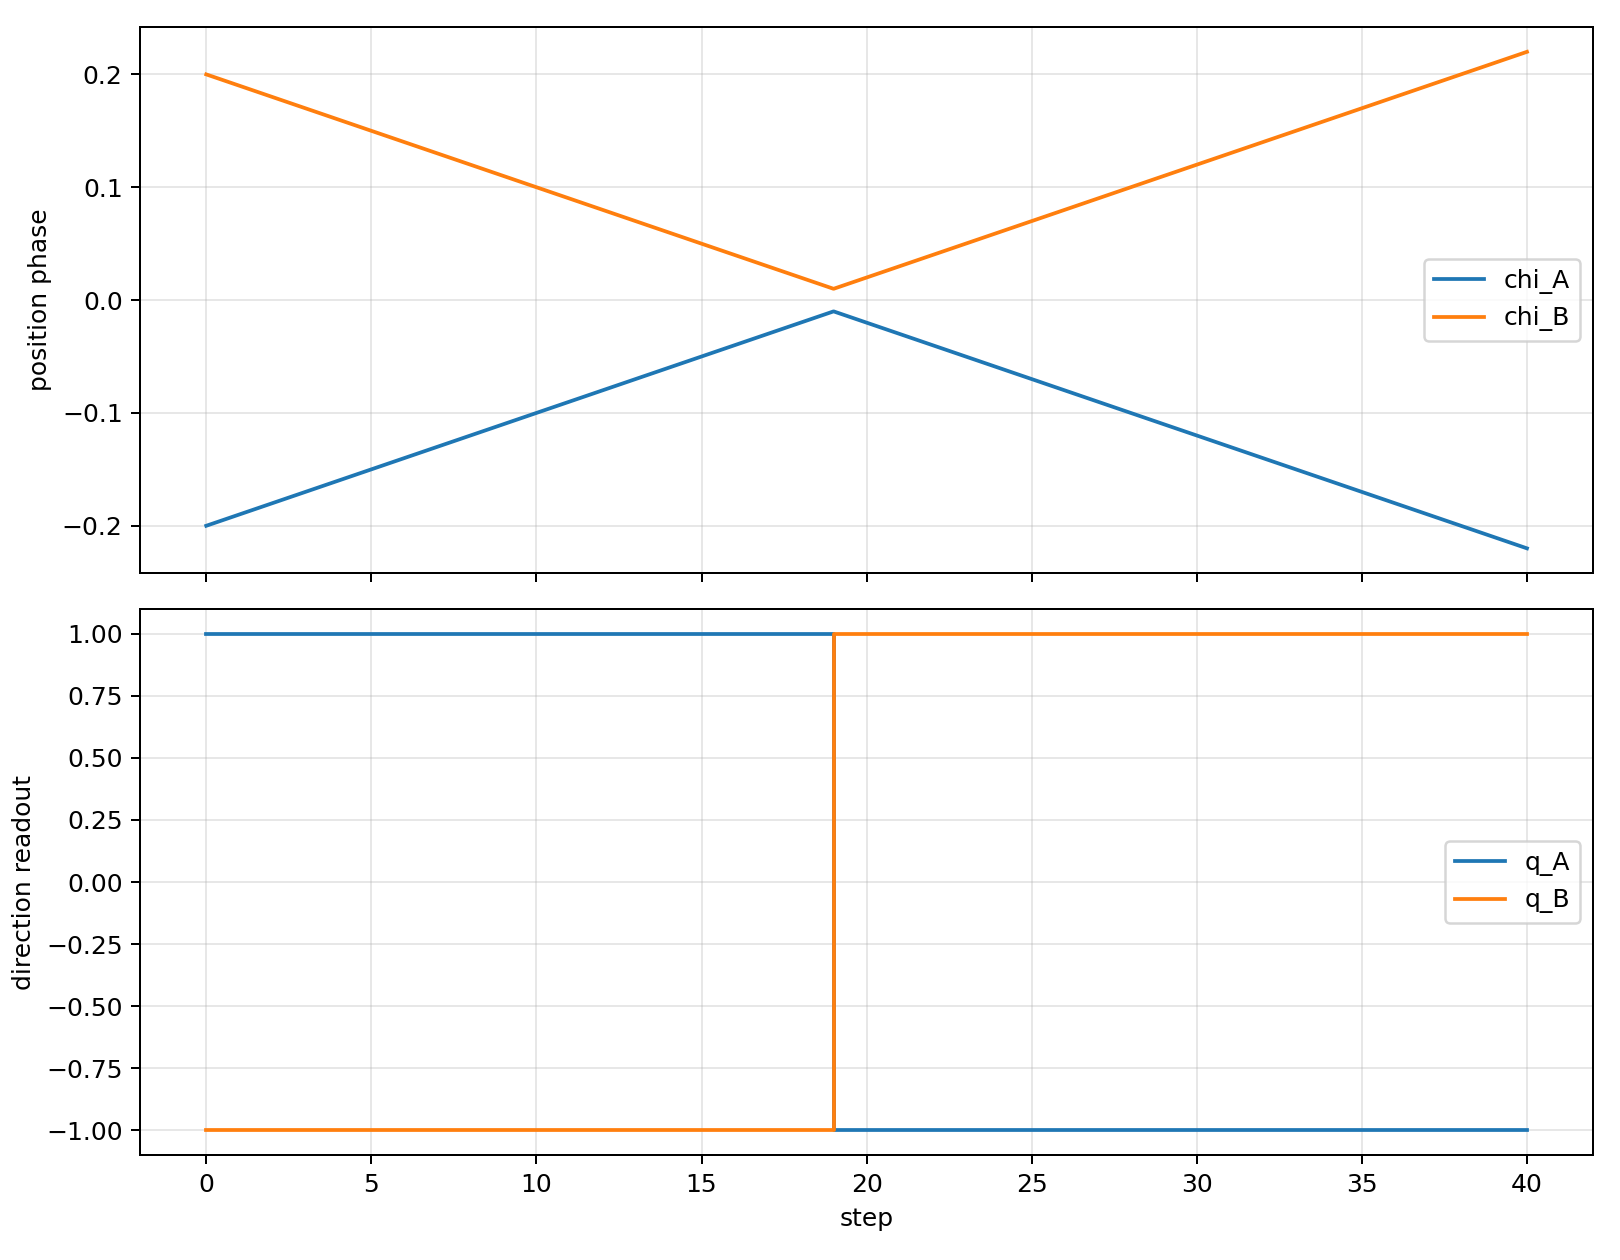
\includegraphics[keepaspectratio,alt={Basic collision trajectory}]{elastic_collision_simulation_result_v2/elastic_collision_trajectory_v2.png}}
\caption{Basic collision trajectory}
\end{figure}

\textbf{Figure 2. Readout of identification oscillation modes}

\begin{figure}
\centering
\pandocbounded{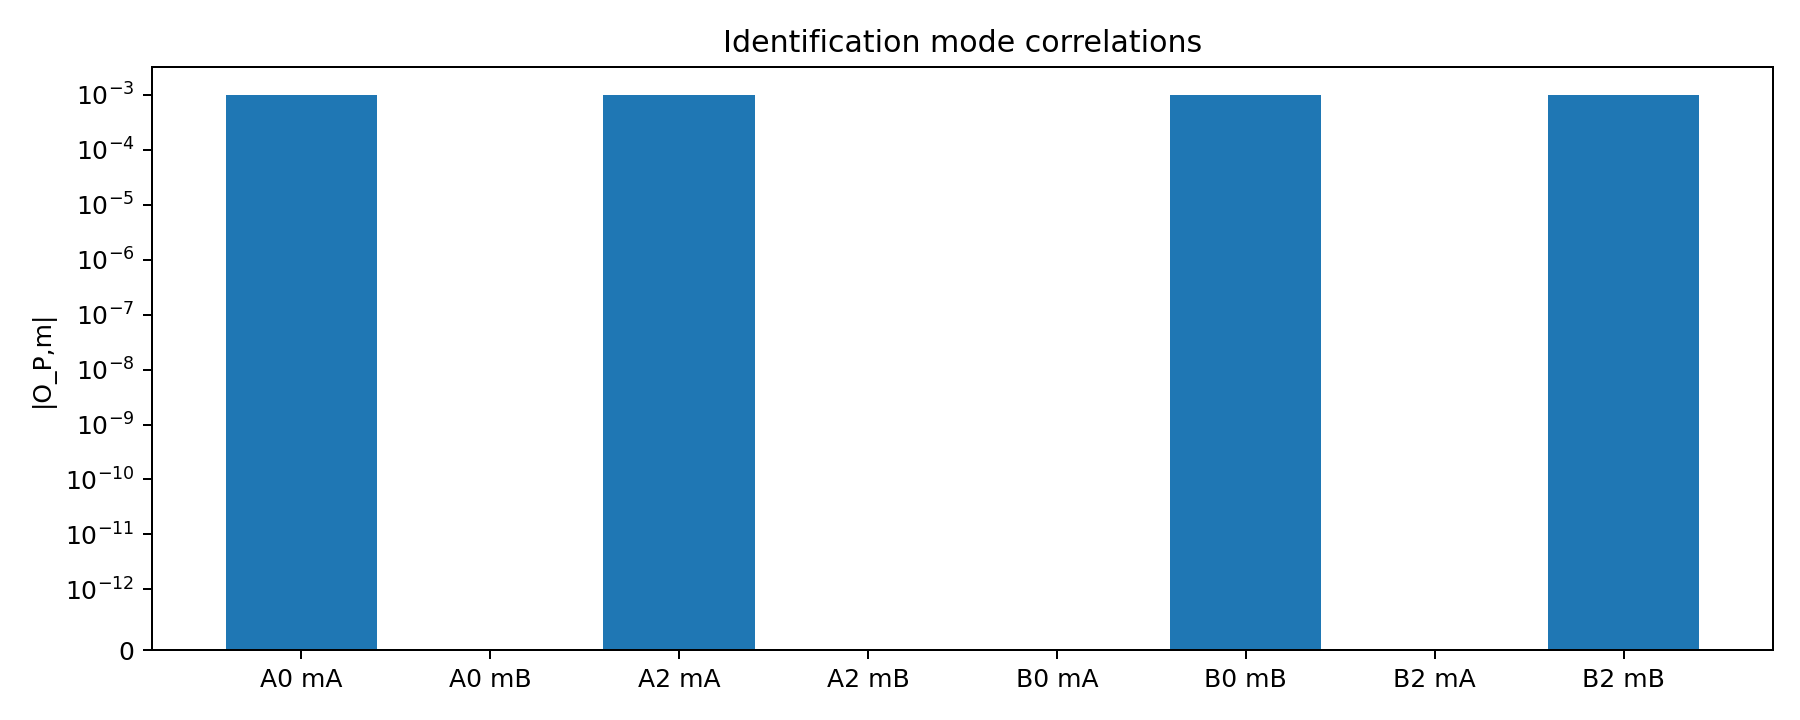
\includegraphics[keepaspectratio,alt={Identification mode readout}]{elastic_collision_simulation_result_v2/elastic_collision_identification_modes_v2.png}}
\caption{Identification mode readout}
\end{figure}

\subsubsection{9.2 Robustness of Identification
Oscillation}\label{robustness-of-identification-oscillation}

When leakage was introduced into the identification oscillation, the
identification mode was preserved for small leakage. As leakage
increased, the purity condition failed.

{\def\LTcaptype{none} % do not increment counter
\begin{longtable}[]{@{}lr@{}}
\toprule\noalign{}
Item & Value \\
\midrule\noalign{}
\endhead
\bottomrule\noalign{}
\endlastfoot
Total cases & \texttt{36} \\
Valid cases & \texttt{20} \\
Invalid cases & \texttt{16} \\
First failing leakage rate & \texttt{0.35} \\
\end{longtable}
}

\textbf{Figure 3. Identification oscillation purity}

\begin{figure}
\centering
\pandocbounded{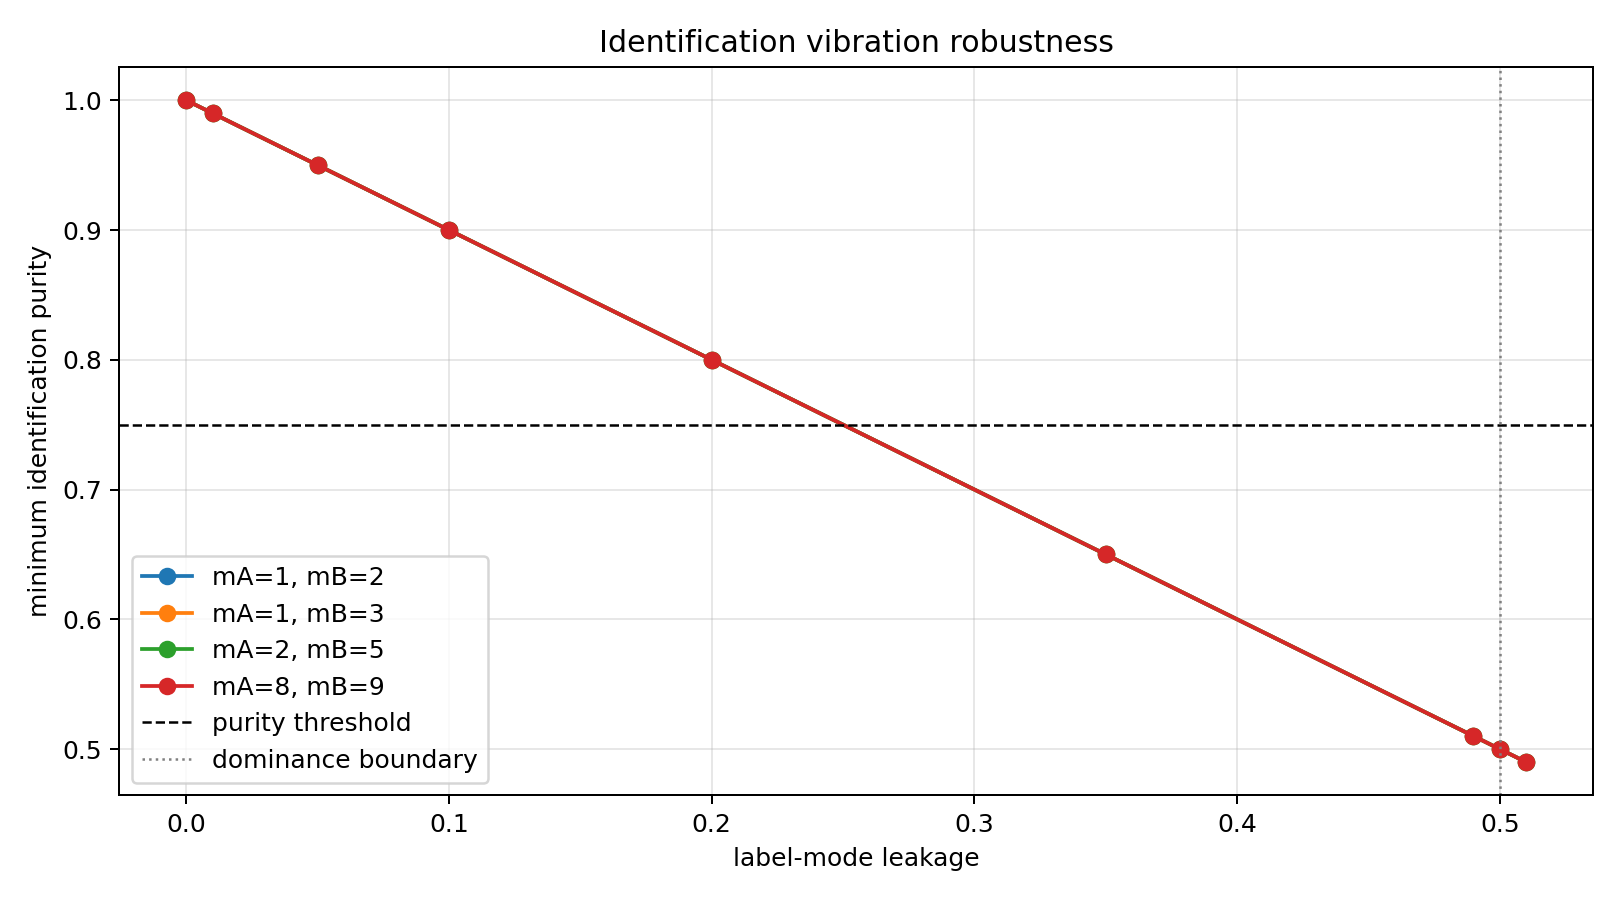
\includegraphics[keepaspectratio,alt={Identification purity}]{elastic_collision_label_robustness_result_v2/label_robustness_purity_v2.png}}
\caption{Identification purity}
\end{figure}

\textbf{Figure 4. Identification preservation verdict}

\begin{figure}
\centering
\pandocbounded{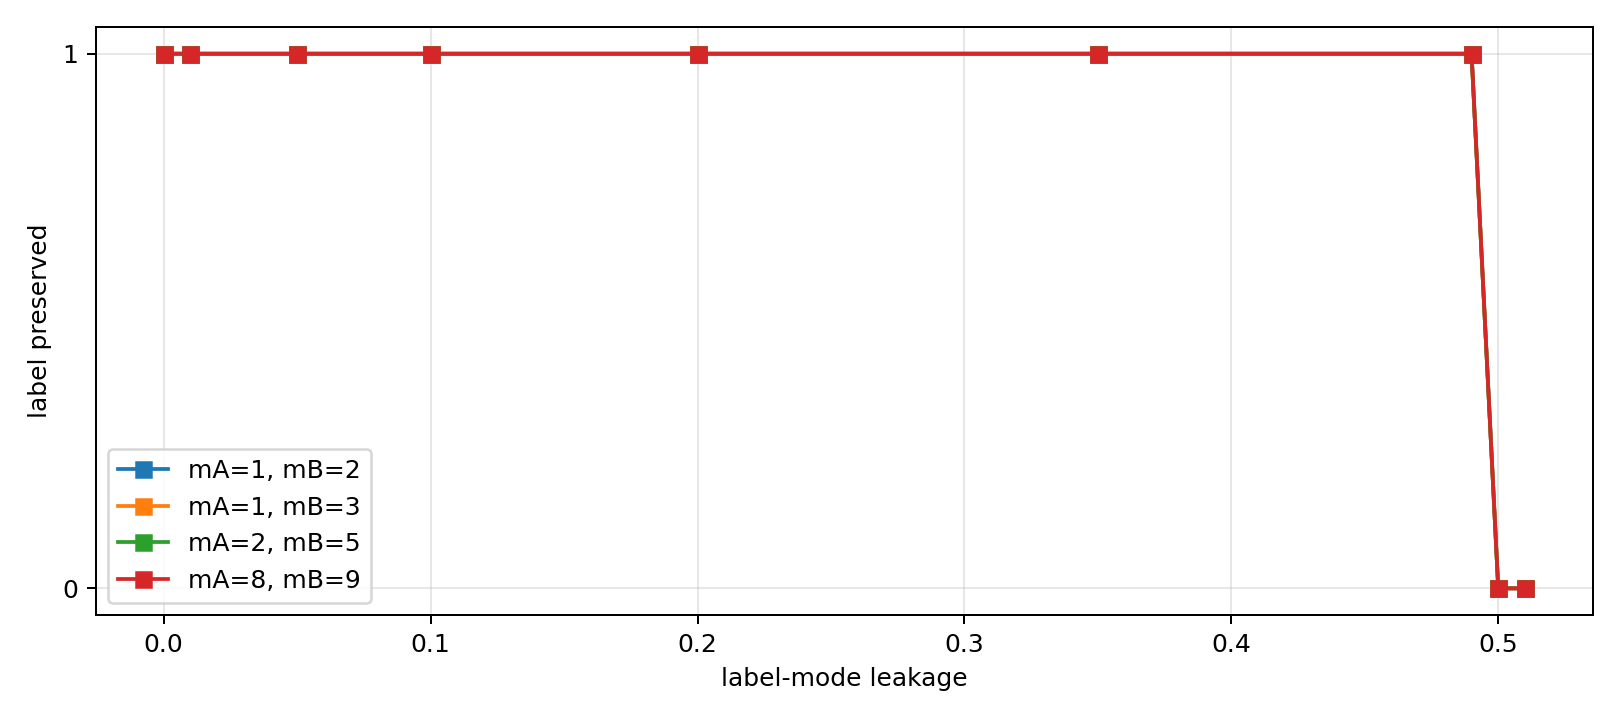
\includegraphics[keepaspectratio,alt={Identification preservation verdict}]{elastic_collision_label_robustness_result_v2/label_robustness_detection_v2.png}}
\caption{Identification preservation verdict}
\end{figure}

\subsubsection{9.3 Heaviness Condition of Observer
C}\label{heaviness-condition-of-observer-c}

When the representative-amplitude capacity of observer \texttt{C} was
too small, the quasi-static condition failed.

{\def\LTcaptype{none} % do not increment counter
\begin{longtable}[]{@{}lr@{}}
\toprule\noalign{}
Item & Value \\
\midrule\noalign{}
\endhead
\bottomrule\noalign{}
\endlastfoot
Total cases & \texttt{13} \\
Valid cases & \texttt{7} \\
Invalid cases & \texttt{6} \\
First valid \texttt{A\_C} & \texttt{20} \\
\end{longtable}
}

\textbf{Figure 5. Observer condition quantities}

\begin{figure}
\centering
\pandocbounded{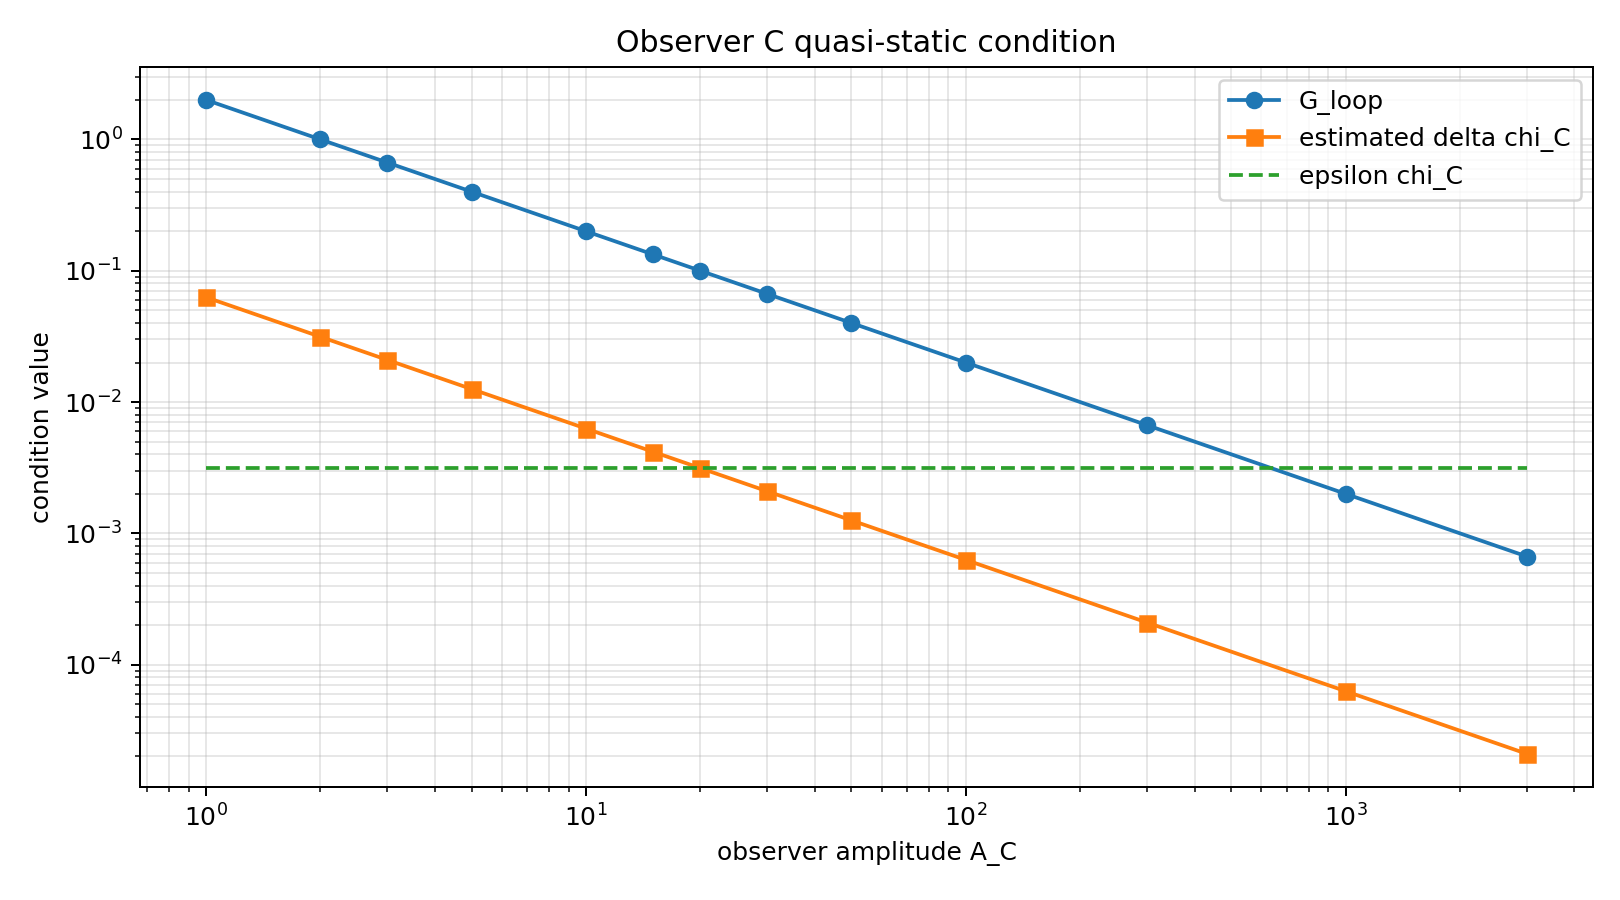
\includegraphics[keepaspectratio,alt={Observer conditions}]{elastic_collision_observer_sweep_result_v2/observer_sweep_conditions_v2.png}}
\caption{Observer conditions}
\end{figure}

\textbf{Figure 6. Validity by observer capacity}

\begin{figure}
\centering
\pandocbounded{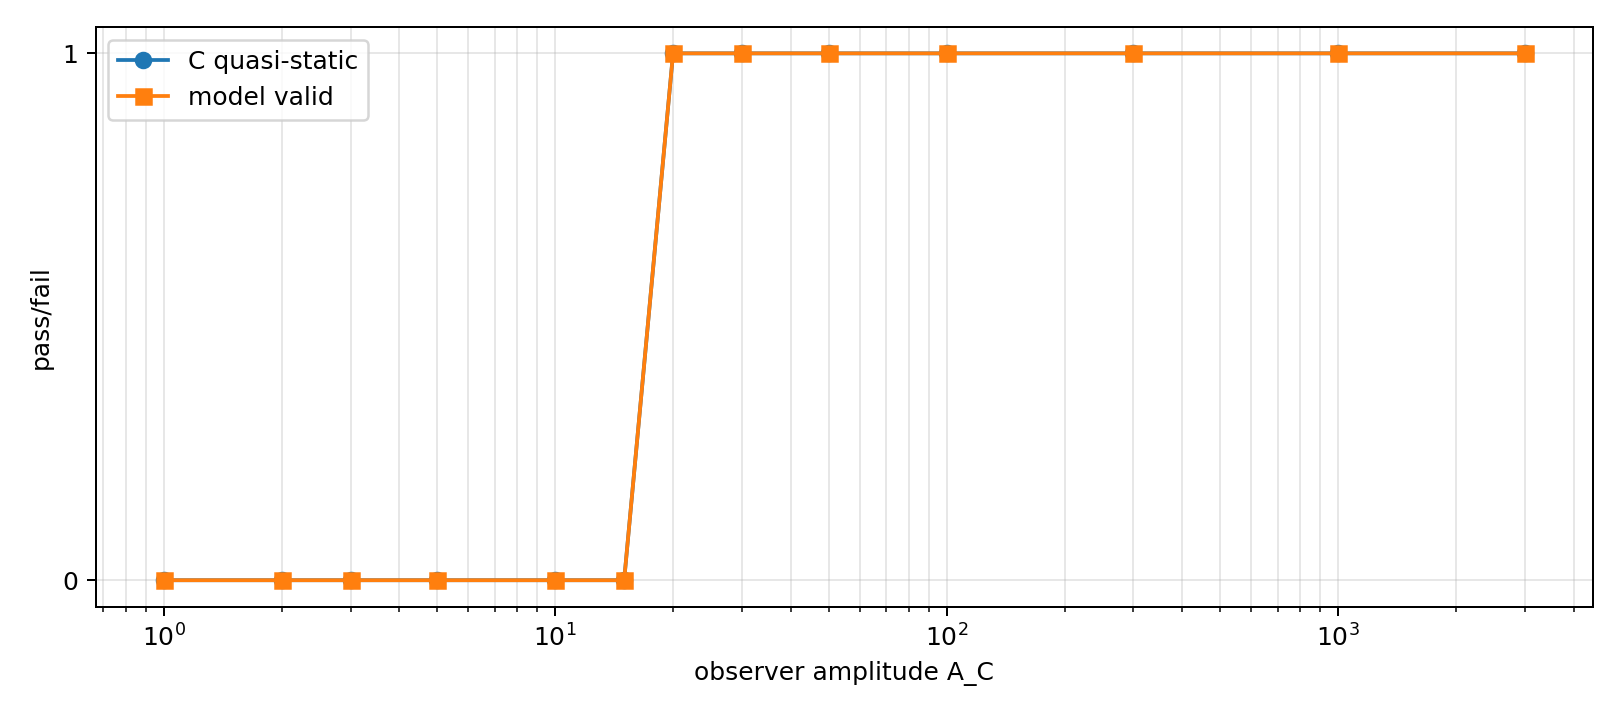
\includegraphics[keepaspectratio,alt={Observer validity}]{elastic_collision_observer_sweep_result_v2/observer_sweep_validity_v2.png}}
\caption{Observer validity}
\end{figure}

\subsubsection{9.4 Cell Resolution and Time
Step}\label{cell-resolution-and-time-step}

When the update step was coarser than the finite cell width, the
collision cell could be skipped.

{\def\LTcaptype{none} % do not increment counter
\begin{longtable}[]{@{}lr@{}}
\toprule\noalign{}
Item & Value \\
\midrule\noalign{}
\endhead
\bottomrule\noalign{}
\endlastfoot
Total cases & \texttt{60} \\
Valid cases & \texttt{57} \\
Invalid cases & \texttt{3} \\
Off-grid valid cases & \texttt{27} \\
Off-grid invalid cases & \texttt{3} \\
\end{longtable}
}

\textbf{Figure 7. Sampling condition}

\begin{figure}
\centering
\pandocbounded{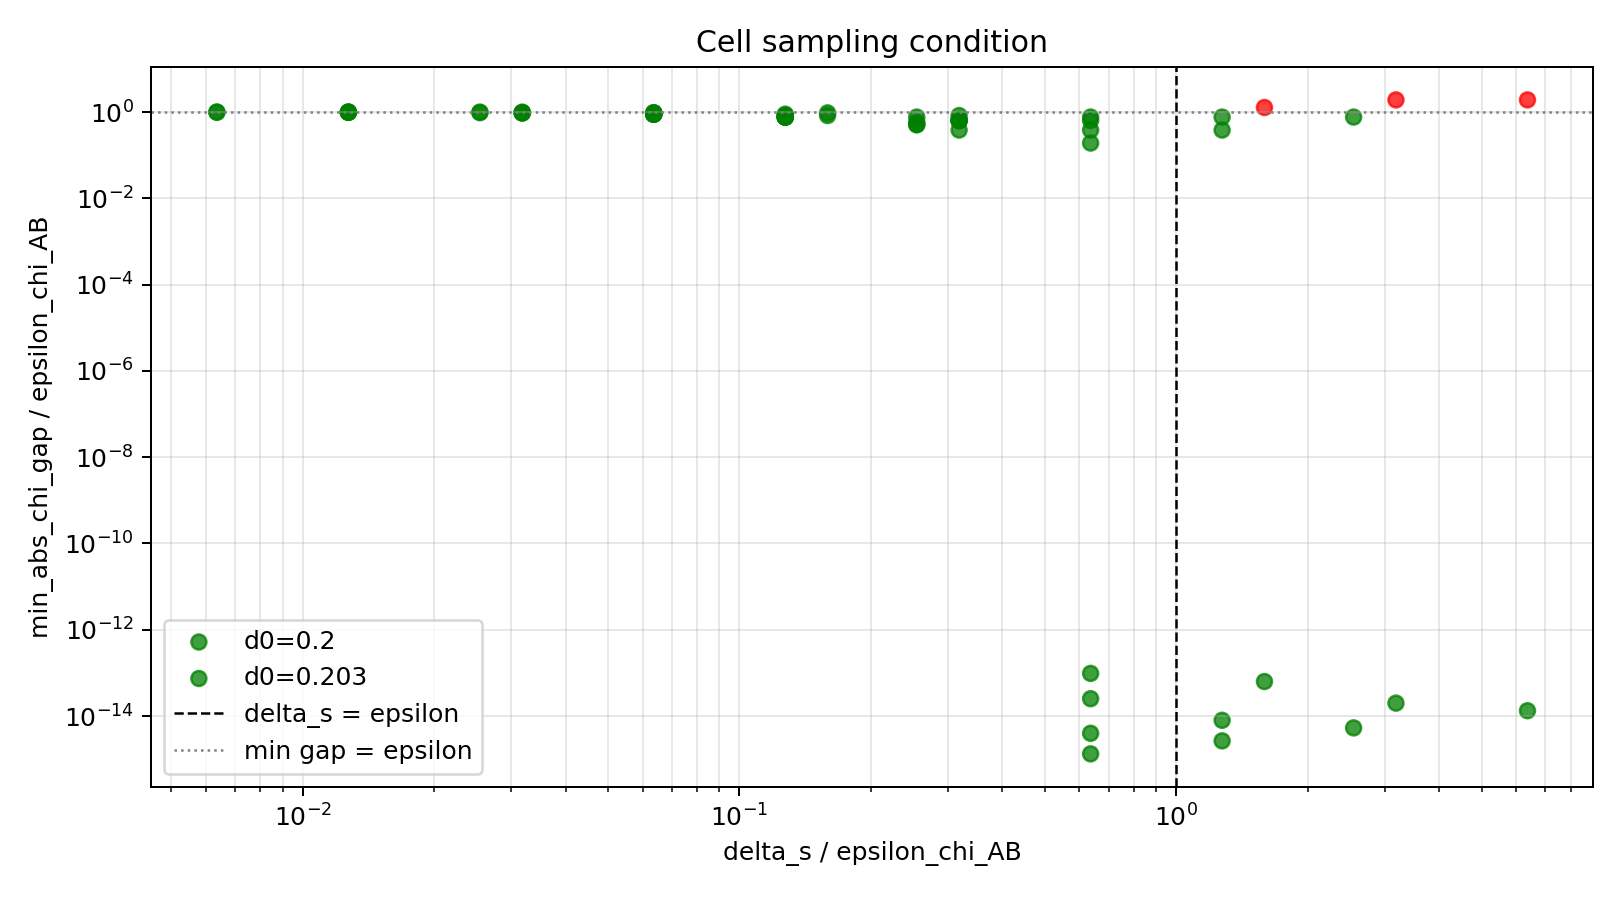
\includegraphics[keepaspectratio,alt={Sampling condition}]{elastic_collision_cell_resolution_sweep_result_v2/cell_resolution_sampling_condition_v2.png}}
\caption{Sampling condition}
\end{figure}

\textbf{Figure 8. Validity under off-grid conditions}

\begin{figure}
\centering
\pandocbounded{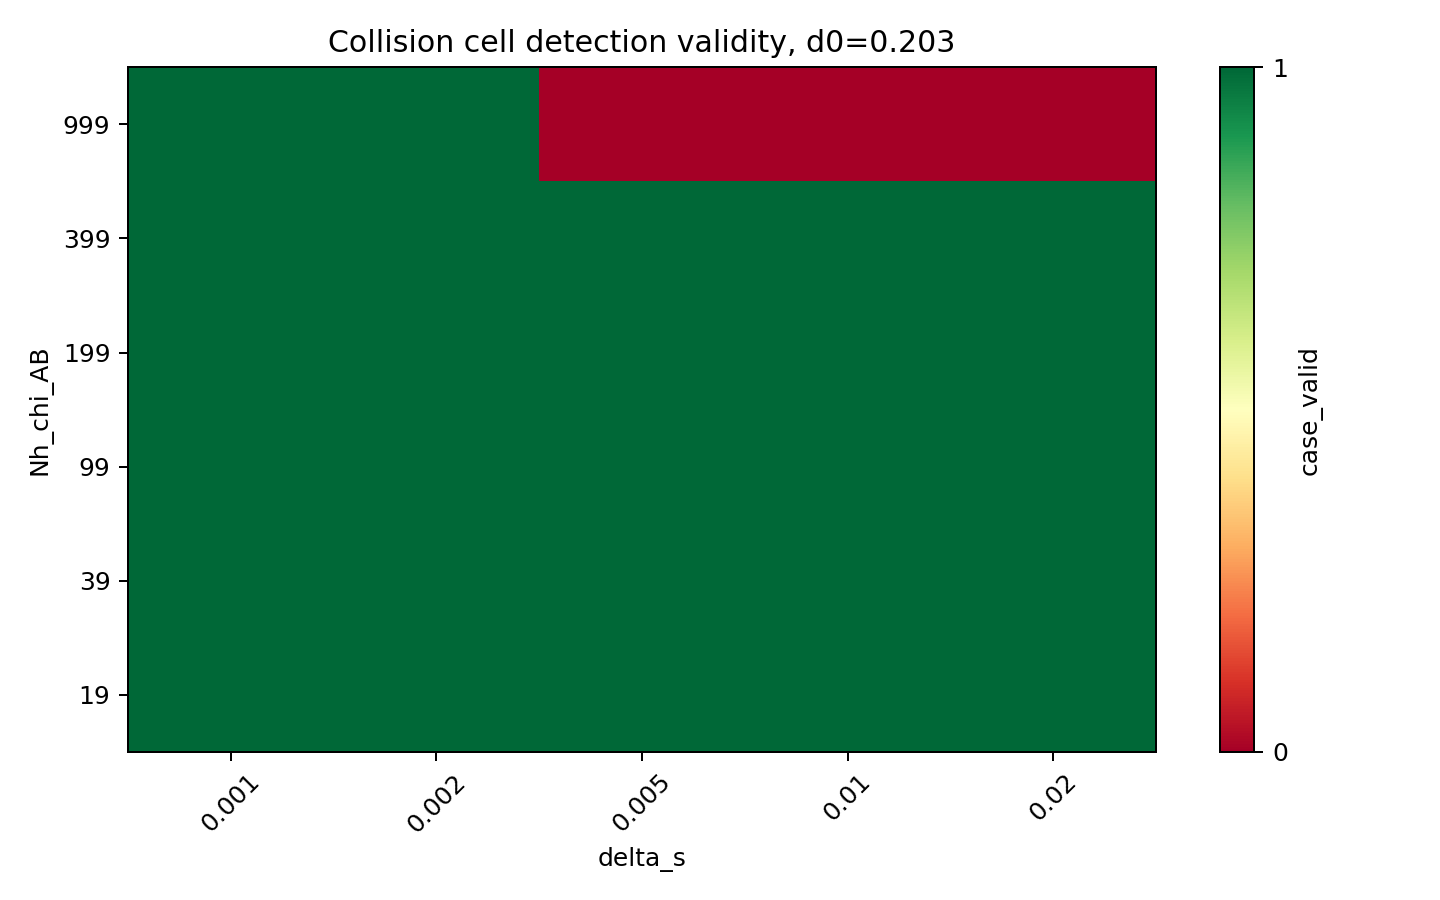
\includegraphics[keepaspectratio,alt={Off-grid validity}]{elastic_collision_cell_resolution_sweep_result_v2/cell_resolution_validity_d0_0_203_v2.png}}
\caption{Off-grid validity}
\end{figure}

\subsubsection{9.5 Control Experiments: Reflection, Transmission, and
Label
Exchange}\label{control-experiments-reflection-transmission-and-label-exchange}

Reflection, transmission, and label-exchange maps were compared.

{\def\LTcaptype{none} % do not increment counter
\begin{longtable}[]{@{}ll@{}}
\toprule\noalign{}
Map & Verdict \\
\midrule\noalign{}
\endhead
\bottomrule\noalign{}
\endlastfoot
reflection & valid \\
transmission & invalid \\
label\_exchange\_reflection & invalid \\
transmission\_with\_label\_exchange & invalid \\
\end{longtable}
}

Only the reflection map simultaneously satisfied direction reversal and
preservation of identification oscillations.

\textbf{Figure 9. Control-map trajectories}

\begin{figure}
\centering
\pandocbounded{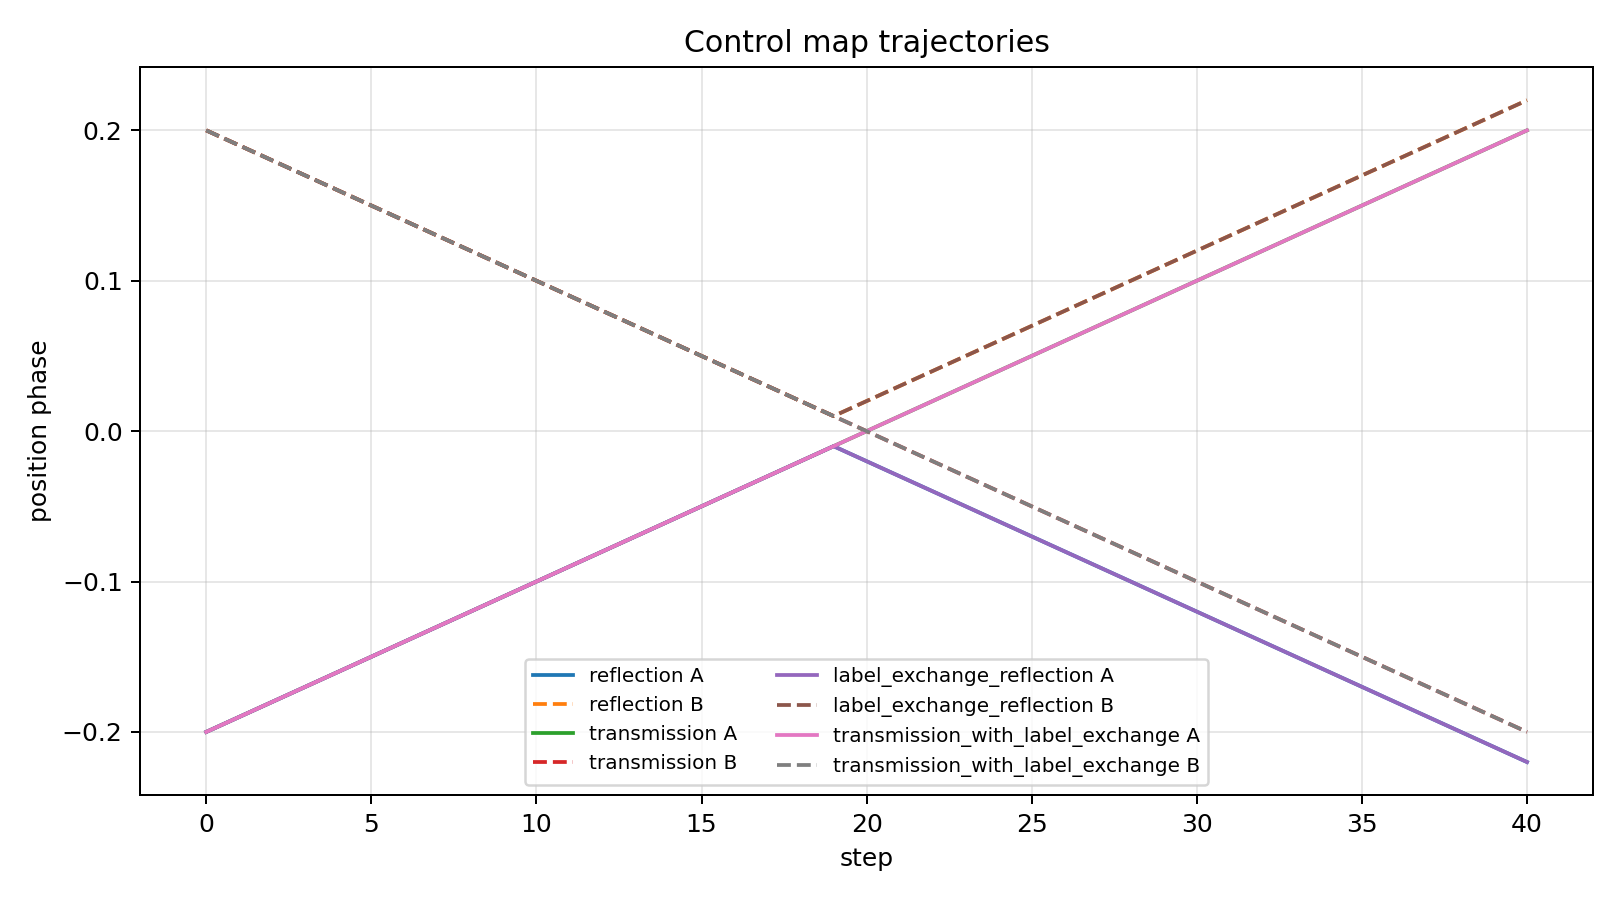
\includegraphics[keepaspectratio,alt={Control map trajectories}]{elastic_collision_control_maps_result_v2/control_maps_trajectories_v2.png}}
\caption{Control map trajectories}
\end{figure}

\textbf{Figure 10. Control-map verdicts}

\begin{figure}
\centering
\pandocbounded{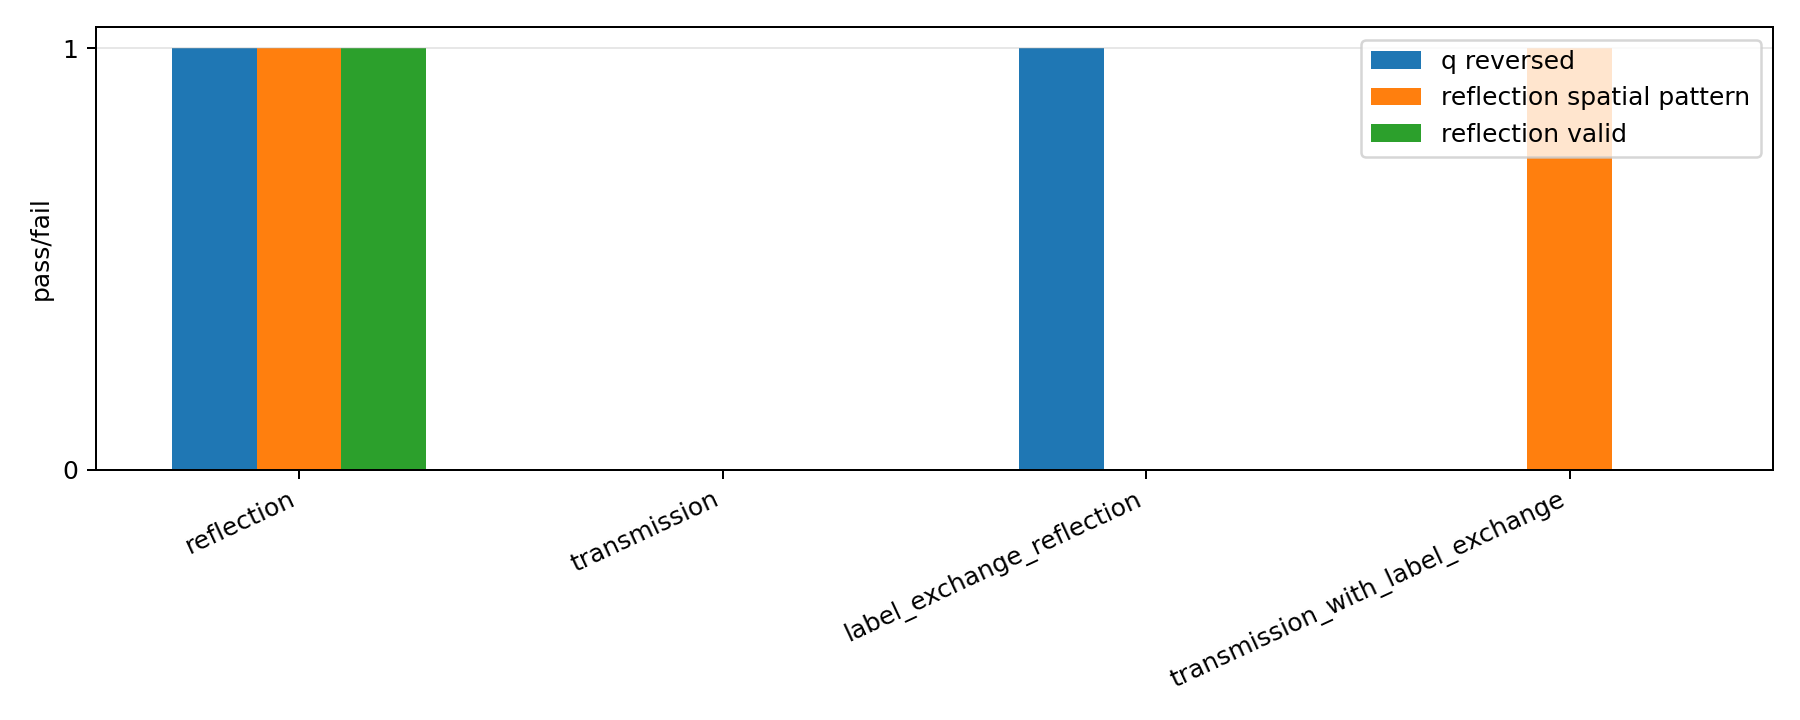
\includegraphics[keepaspectratio,alt={Control map verdicts}]{elastic_collision_control_maps_result_v2/control_maps_verdict_v2.png}}
\caption{Control map verdicts}
\end{figure}

\subsubsection{9.6 Asymmetric Conditions}\label{asymmetric-conditions}

Amplitude differences and harmonic-order differences alone did not break
the map. The main cause of failure was loss of simultaneous satisfaction
of the spatial and temporal cells.

{\def\LTcaptype{none} % do not increment counter
\begin{longtable}[]{@{}lr@{}}
\toprule\noalign{}
Item & Value \\
\midrule\noalign{}
\endhead
\bottomrule\noalign{}
\endlastfoot
Total cases & \texttt{10} \\
Valid cases & \texttt{7} \\
Invalid cases & \texttt{3} \\
\end{longtable}
}

\textbf{Figure 11. Cell gaps under asymmetric conditions}

\begin{figure}
\centering
\pandocbounded{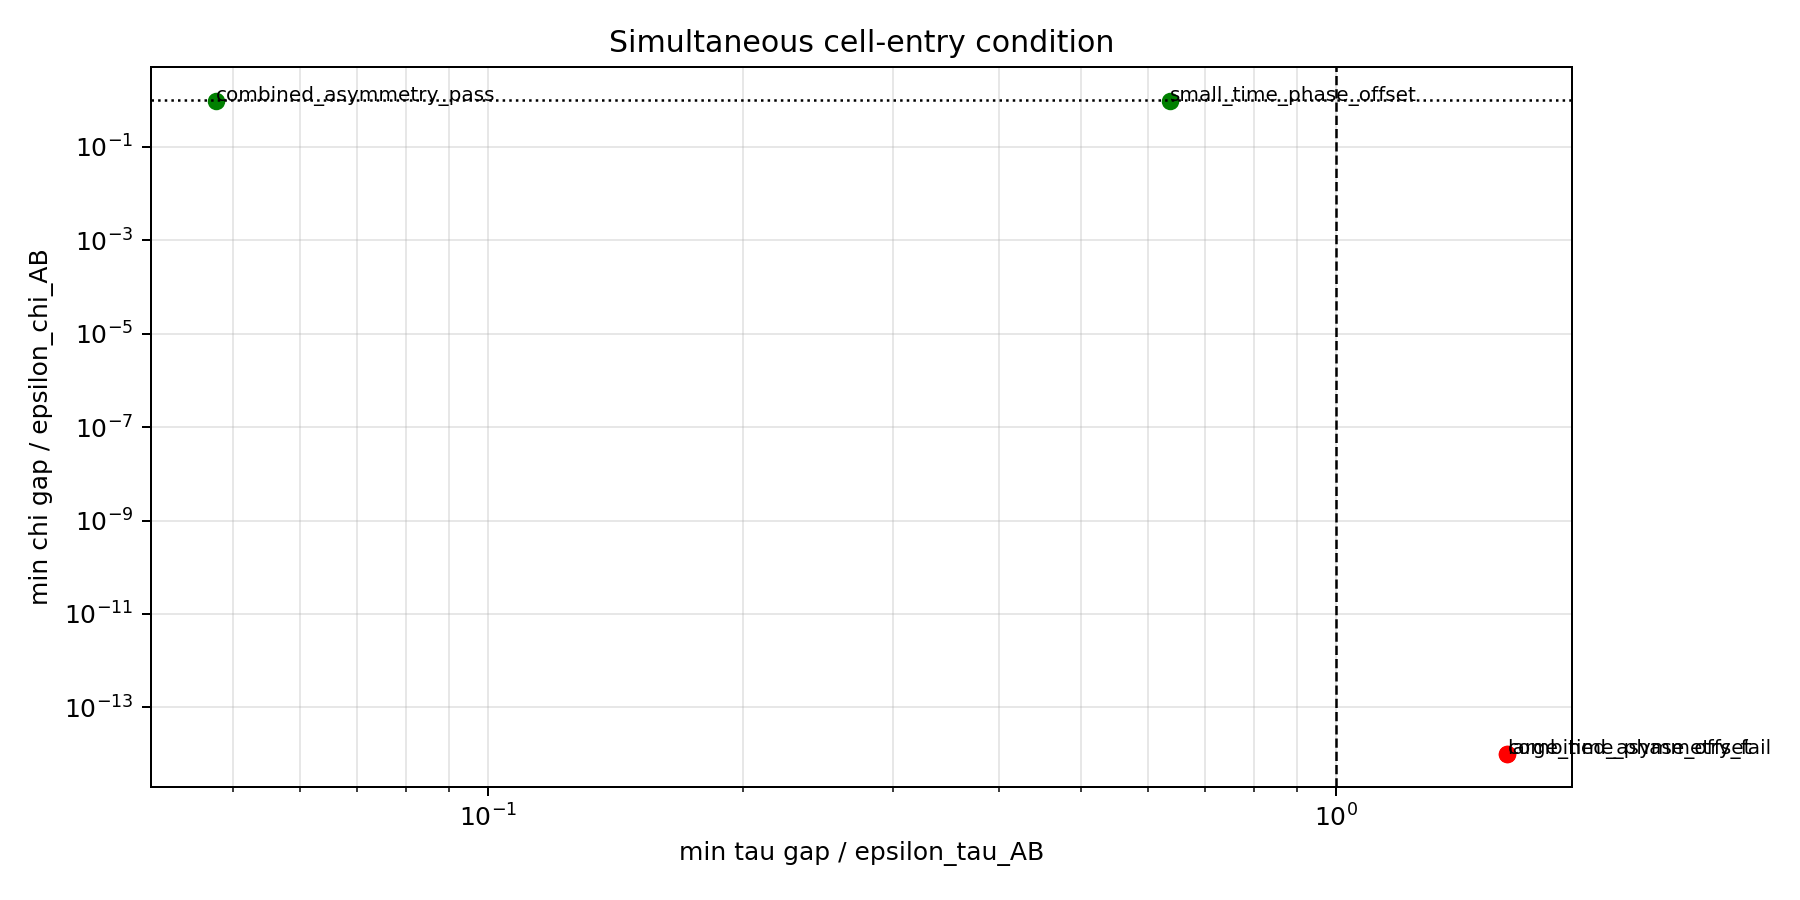
\includegraphics[keepaspectratio,alt={Asymmetric cell gaps}]{elastic_collision_asymmetry_sweep_result_v2/asymmetry_sweep_cell_gaps_v2.png}}
\caption{Asymmetric cell gaps}
\end{figure}

\textbf{Figure 12. Asymmetry verdicts}

\begin{figure}
\centering
\pandocbounded{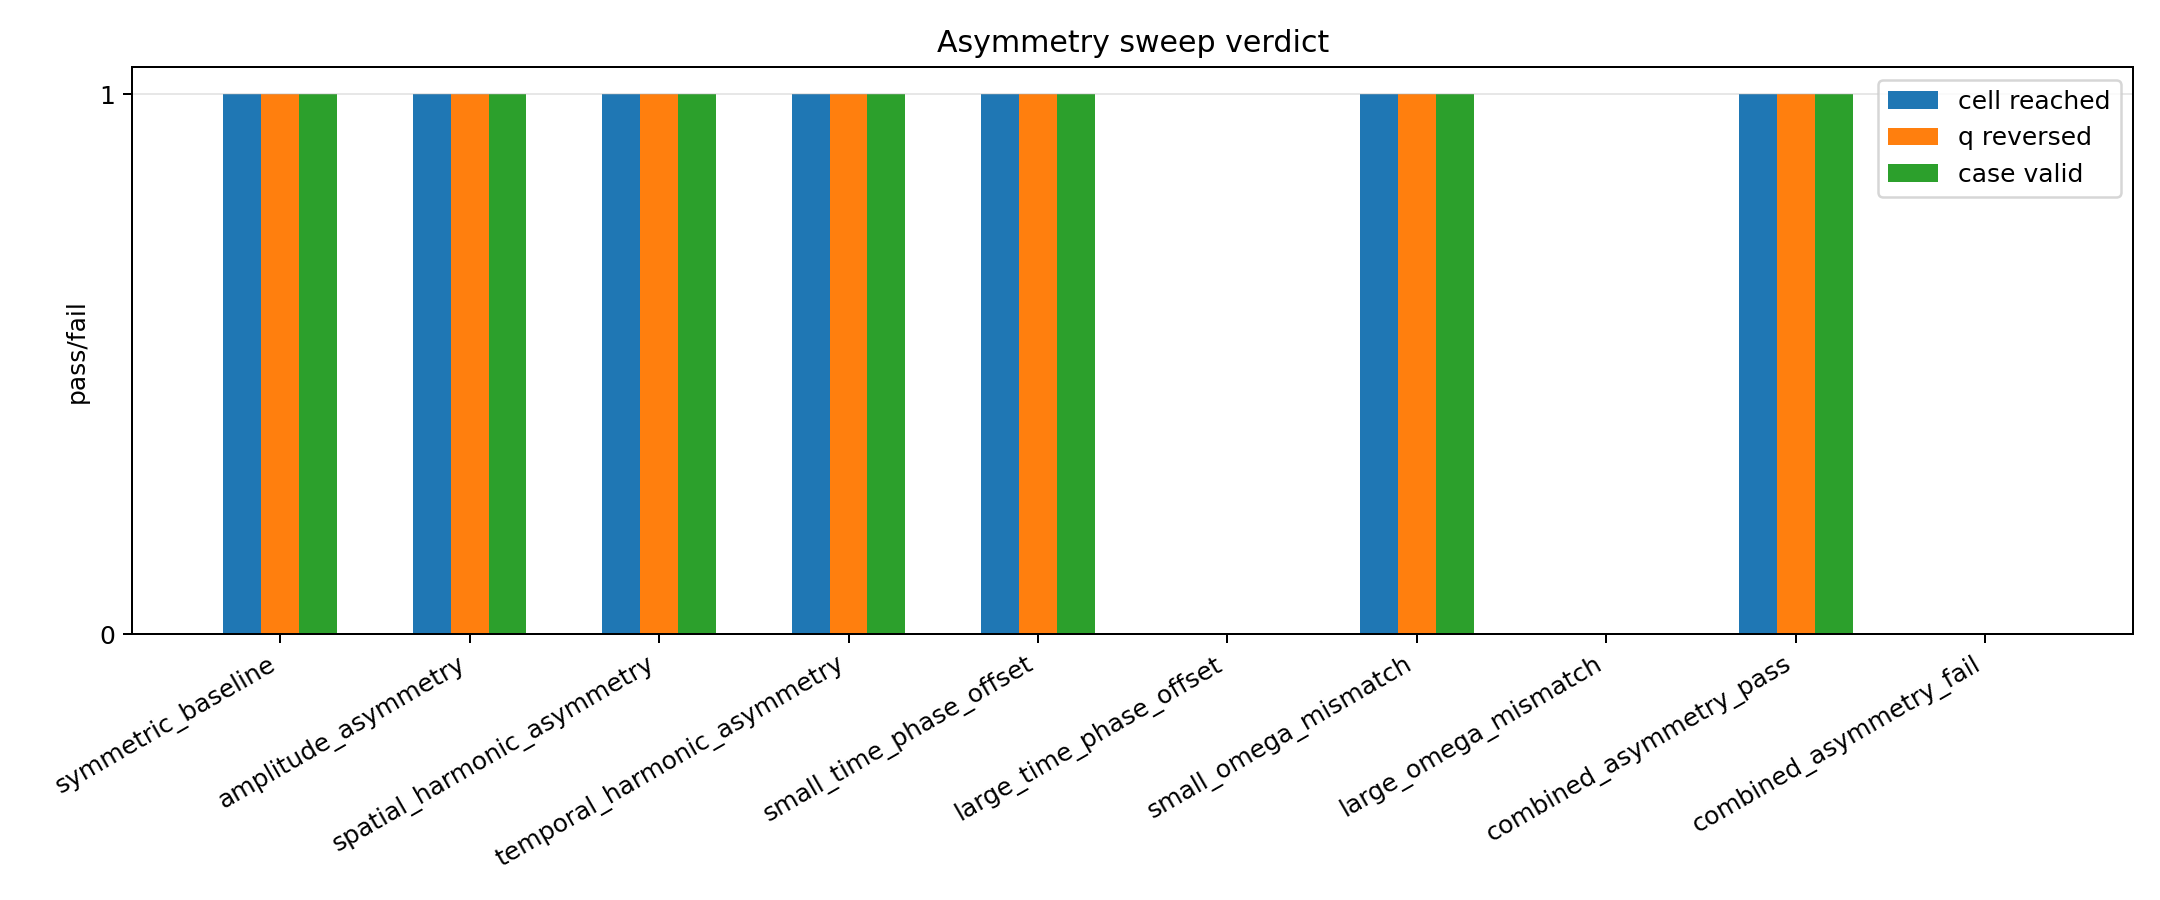
\includegraphics[keepaspectratio,alt={Asymmetry verdicts}]{elastic_collision_asymmetry_sweep_result_v2/asymmetry_sweep_verdict_v2.png}}
\caption{Asymmetry verdicts}
\end{figure}

\subsubsection{9.7 Observation
Perturbation}\label{observation-perturbation}

When observation perturbation exceeded the localization width of
\texttt{C}, the observation model failed. However, as long as the AB
cell condition was satisfied, the collision map itself could still hold.

{\def\LTcaptype{none} % do not increment counter
\begin{longtable}[]{@{}lr@{}}
\toprule\noalign{}
Item & Value \\
\midrule\noalign{}
\endhead
\bottomrule\noalign{}
\endlastfoot
Total cases & \texttt{8} \\
Observation-model valid cases & \texttt{5} \\
Collision-map valid cases & \texttt{7} \\
Invalid cases & \texttt{3} \\
\end{longtable}
}

\textbf{Figure 13. Observation perturbation thresholds}

\begin{figure}
\centering
\pandocbounded{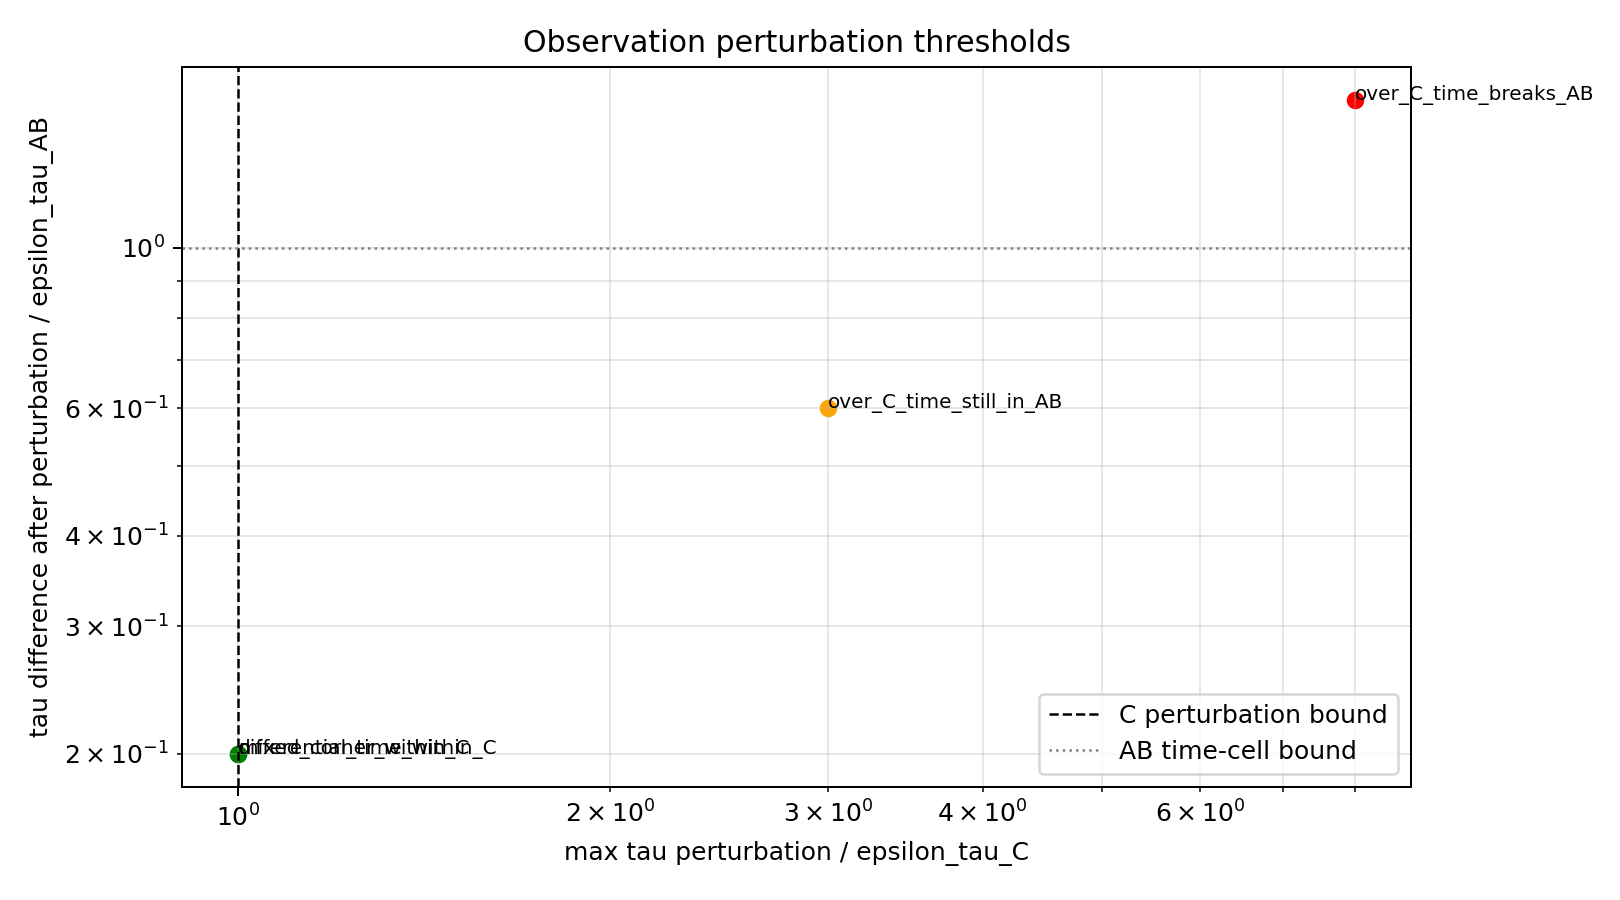
\includegraphics[keepaspectratio,alt={Observation perturbation thresholds}]{elastic_collision_observation_perturbation_result_v2/observation_perturbation_thresholds_v2.png}}
\caption{Observation perturbation thresholds}
\end{figure}

\textbf{Figure 14. Observation perturbation verdicts}

\begin{figure}
\centering
\pandocbounded{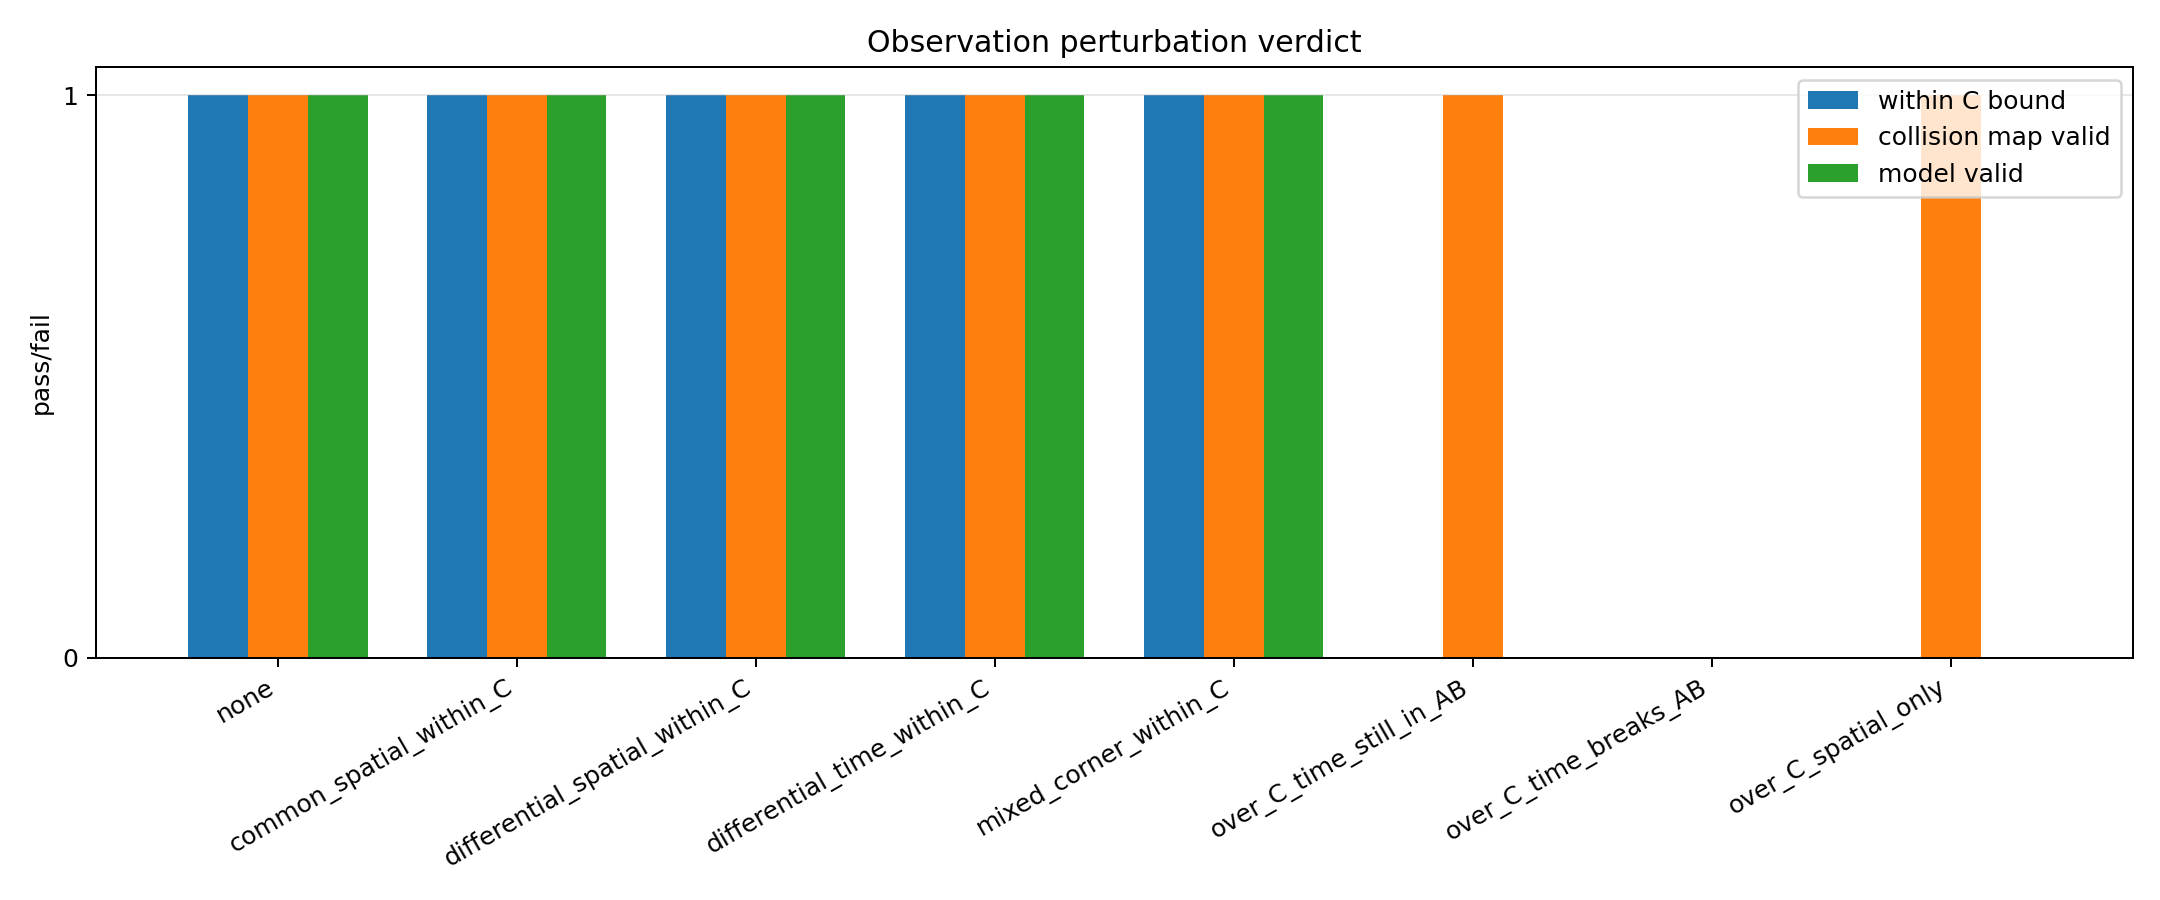
\includegraphics[keepaspectratio,alt={Observation perturbation verdicts}]{elastic_collision_observation_perturbation_result_v2/observation_perturbation_verdict_v2.png}}
\caption{Observation perturbation verdicts}
\end{figure}

\subsubsection{9.8 Multiple Collisions}\label{multiple-collisions}

Within a closed interval, wall reflections were allowed and AB
collisions were repeated.

{\def\LTcaptype{none} % do not increment counter
\begin{longtable}[]{@{}lr@{}}
\toprule\noalign{}
Item & Value \\
\midrule\noalign{}
\endhead
\bottomrule\noalign{}
\endlastfoot
Target AB collisions & \texttt{8} \\
Actual AB collisions & \texttt{8} \\
Wall reflections & \texttt{14} \\
All identification modes preserved & \texttt{true} \\
\texttt{q} reversed at each collision & \texttt{true} \\
Representative amplitudes preserved & \texttt{true} \\
Closure preserved & \texttt{true} \\
Overall verdict & \texttt{true} \\
\end{longtable}
}

\textbf{Figure 15. Trajectories in repeated collisions}

\begin{figure}
\centering
\pandocbounded{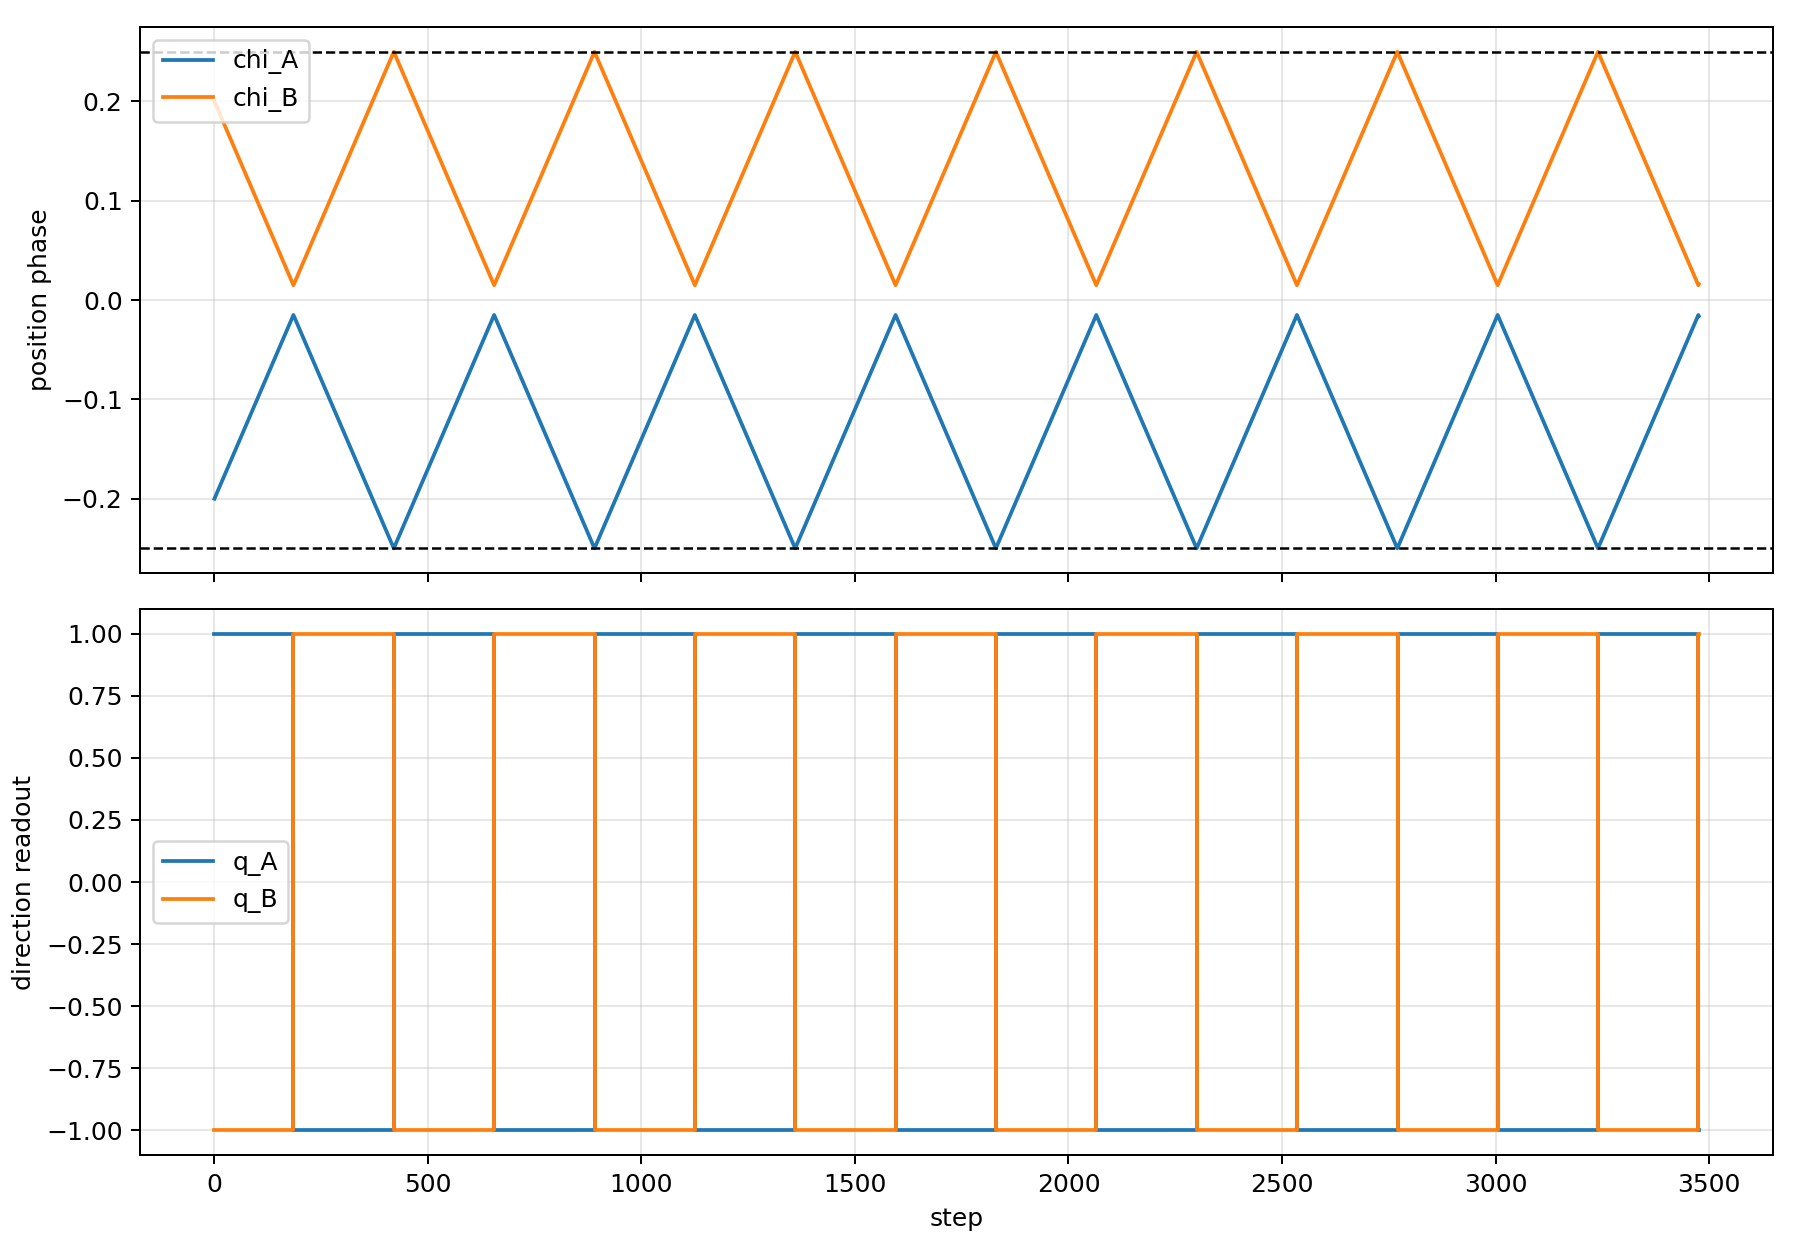
\includegraphics[keepaspectratio,alt={Multiple collision trajectory}]{elastic_collision_multi_collision_result_v2/multi_collision_trajectory_v2.png}}
\caption{Multiple collision trajectory}
\end{figure}

\textbf{Figure 16. Closure residual in repeated collisions}

\begin{figure}
\centering
\pandocbounded{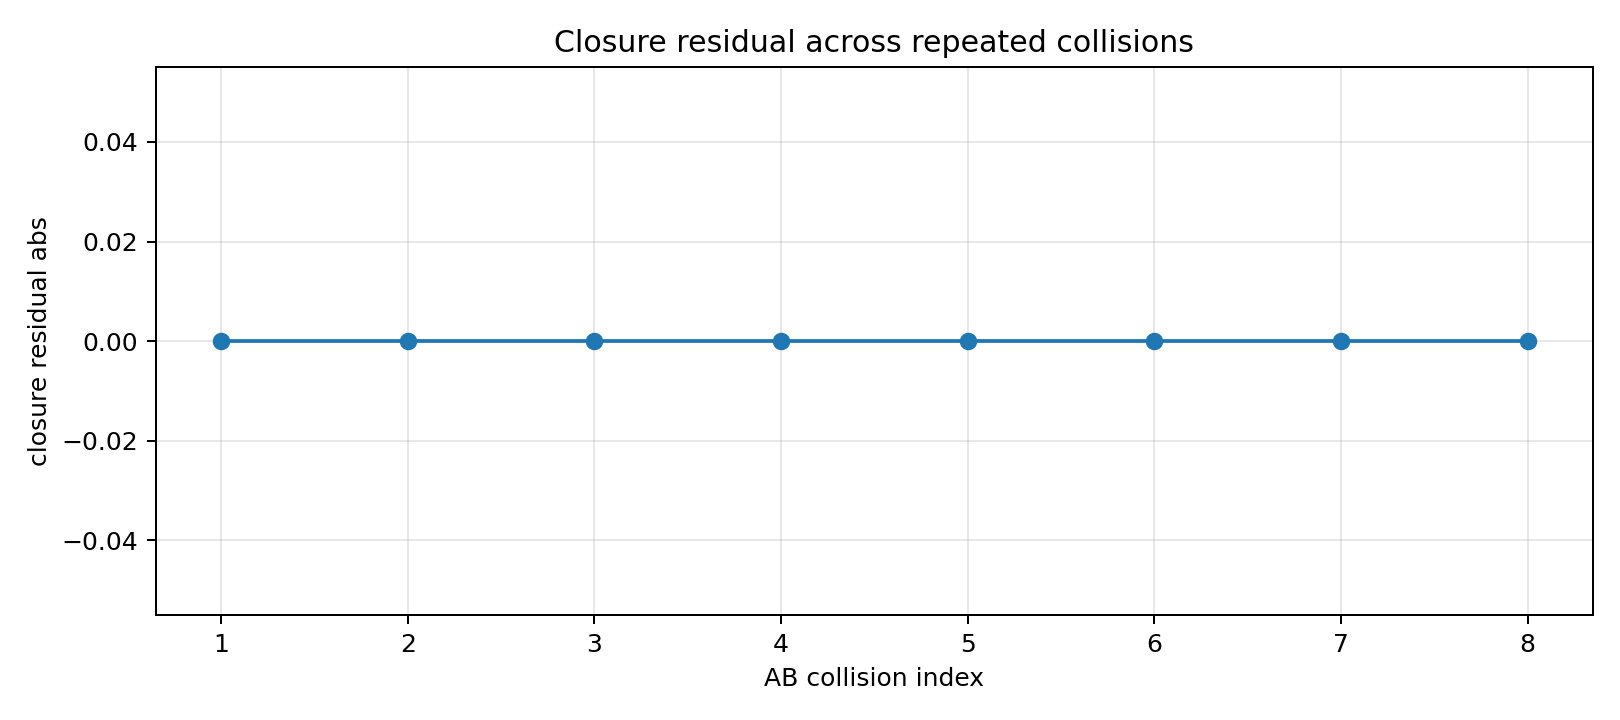
\includegraphics[keepaspectratio,alt={Multiple collision closure residual}]{elastic_collision_multi_collision_result_v2/multi_collision_closure_v2.png}}
\caption{Multiple collision closure residual}
\end{figure}

\subsubsection{\texorpdfstring{9.9 Readout Resolution of \texttt{η}
Identification
Oscillation}{9.9 Readout Resolution of η Identification Oscillation}}\label{readout-resolution-of-ux3b7-identification-oscillation}

When the internal identification oscillation was read with a finite
number of samples, aliasing occurred if the mode difference was a
multiple of the sample count.

{\def\LTcaptype{none} % do not increment counter
\begin{longtable}[]{@{}lr@{}}
\toprule\noalign{}
Item & Value \\
\midrule\noalign{}
\endhead
\bottomrule\noalign{}
\endlastfoot
Total cases & \texttt{88} \\
Valid cases & \texttt{59} \\
Invalid cases & \texttt{29} \\
Aliasing cases & \texttt{29} \\
Non-aliasing failures & \texttt{0} \\
Minimum \texttt{η} sample count valid for all mode pairs &
\texttt{64} \\
\end{longtable}
}

All invalid cases were due to \texttt{η} readout aliasing. This is not a
failure of the collision map itself, but insufficient readout resolution
for the identification oscillation.

\textbf{Figure 17. Validity of \texttt{η} readout resolution}

\begin{figure}
\centering
\pandocbounded{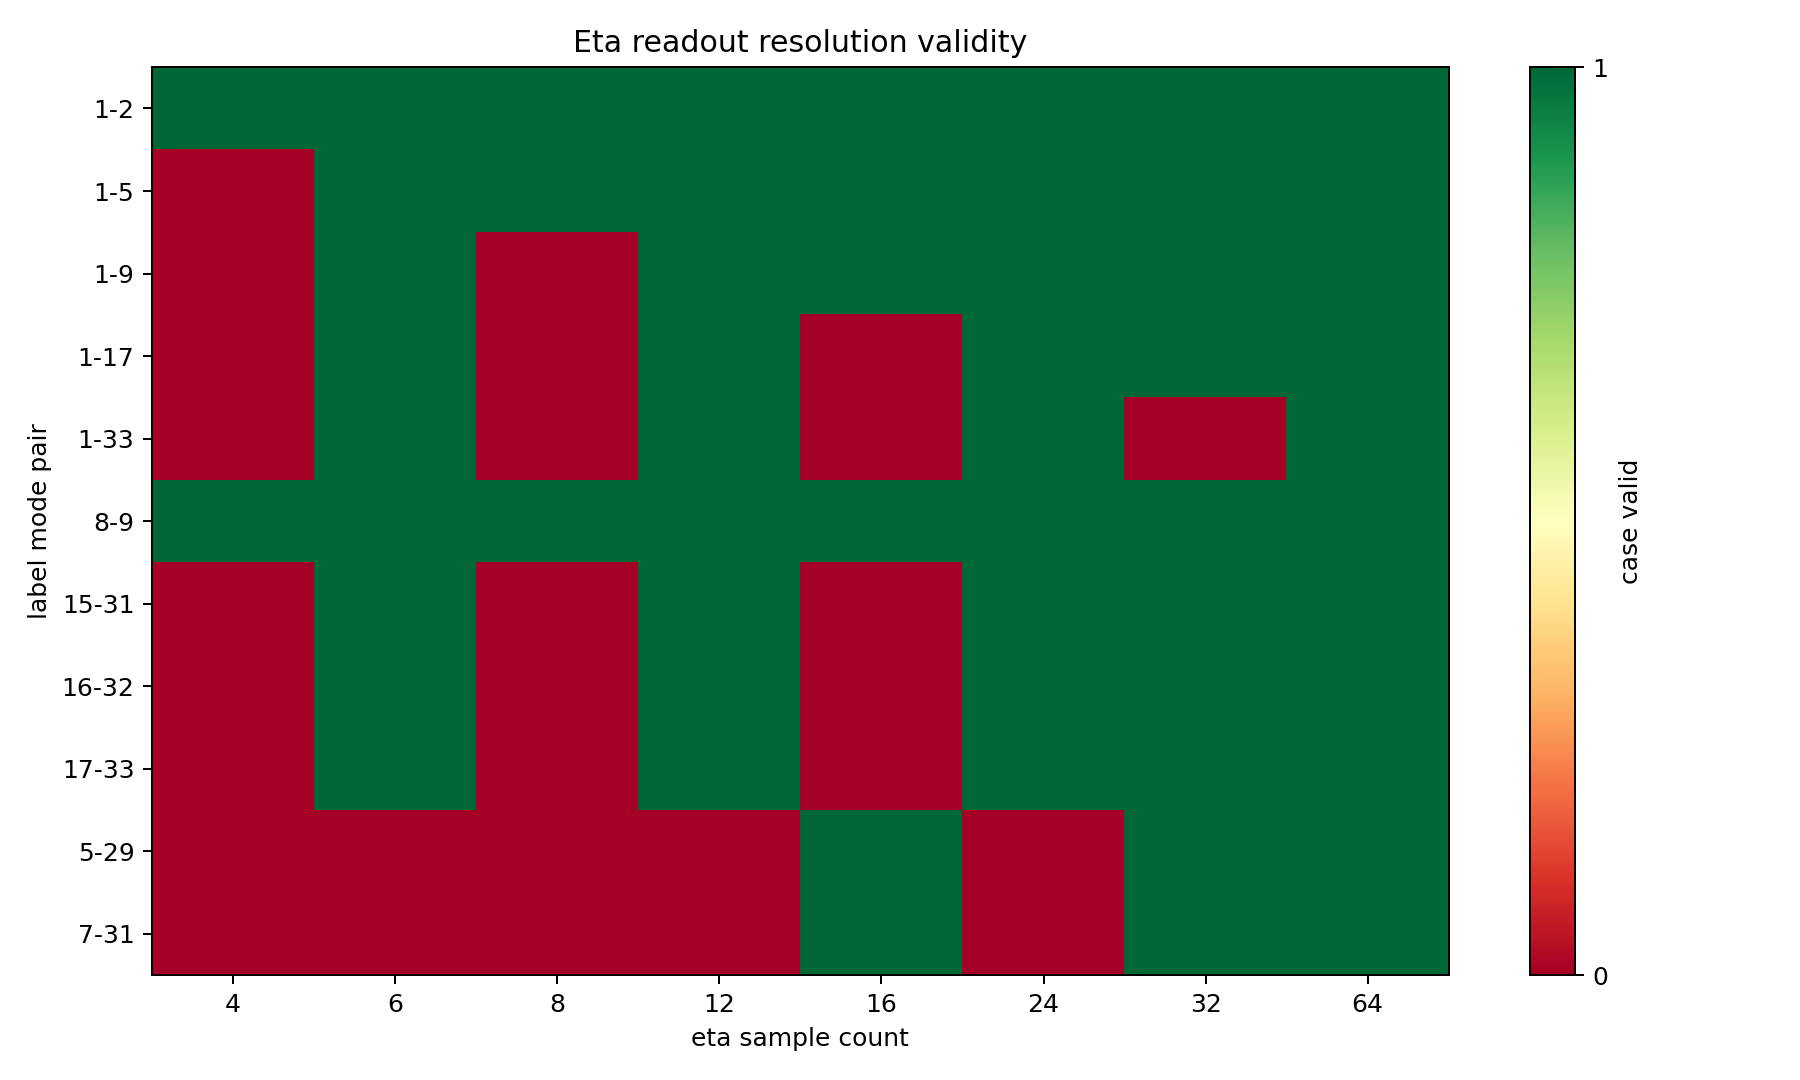
\includegraphics[keepaspectratio,alt={Eta validity}]{elastic_collision_eta_resolution_sweep_result_v2/eta_resolution_validity_v2.png}}
\caption{Eta validity}
\end{figure}

\textbf{Figure 18. \texttt{η} identification purity}

\begin{figure}
\centering
\pandocbounded{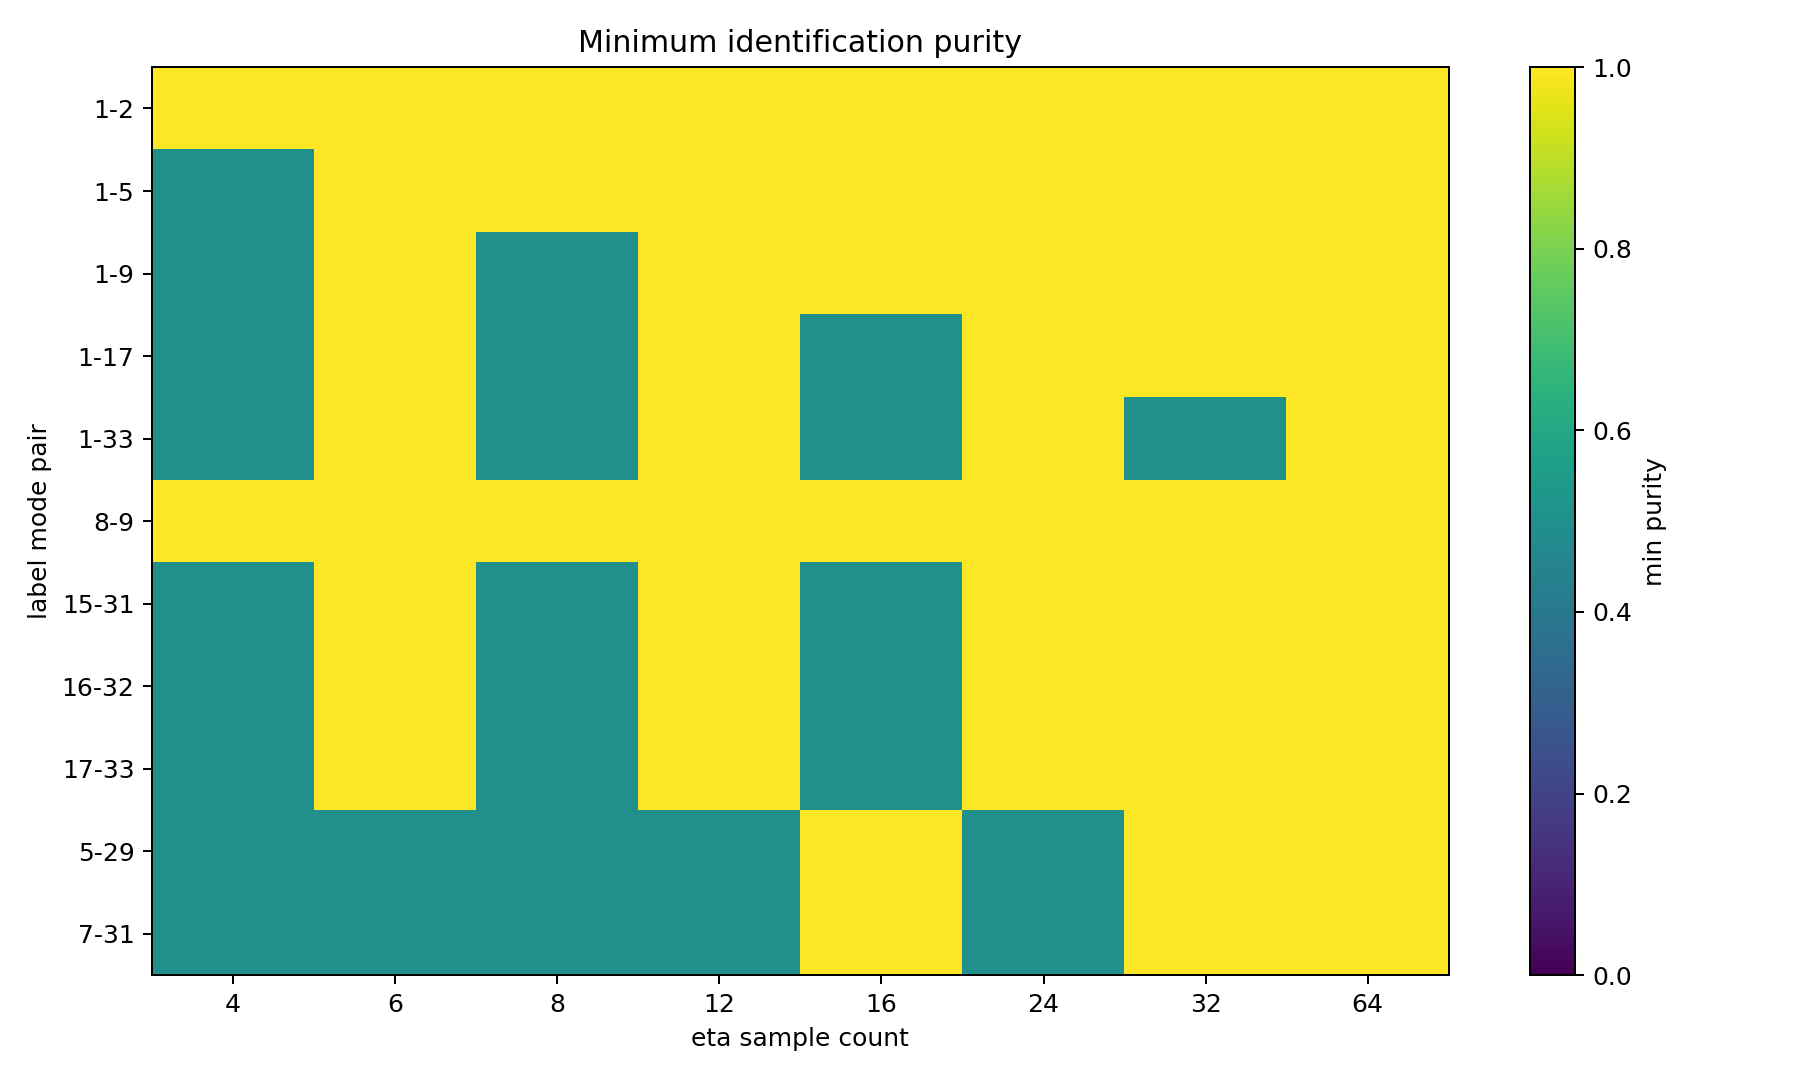
\includegraphics[keepaspectratio,alt={Eta purity}]{elastic_collision_eta_resolution_sweep_result_v2/eta_resolution_purity_v2.png}}
\caption{Eta purity}
\end{figure}

\begin{center}\rule{0.5\linewidth}{0.5pt}\end{center}

\subsection{10. Discussion}\label{discussion}

\subsubsection{10.1 Distinguishing Reflection from
Transmission}\label{distinguishing-reflection-from-transmission}

If one observes only position trajectories, reflection and transmission
can often be difficult to distinguish. This paper tracks the
identification oscillations \texttt{m\_A,m\_B} and the direction
readouts \texttt{q\_A,q\_B} simultaneously.

Transmission and label-exchange maps can resemble reflection at the
level of position readout, but are rejected by the conditions of
direction reversal or identification-mode preservation.

Thus the reflection criterion is not merely an apparent trajectory. It
includes the condition:

\begin{Shaded}
\begin{Highlighting}[]
\NormalTok{the local wave carrying its identification oscillation is pushed out in the reversed direction}
\end{Highlighting}
\end{Shaded}

\subsubsection{10.2 Local Interaction Without Background
Space}\label{local-interaction-without-background-space}

This paper does not place background space at the start. Position is
treated not as an external spatial coordinate, but as a relative-phase
readout with respect to the observer.

The heavy observer \texttt{C} is not fully solved as a dynamical third
body. Instead, it is absorbed as a quasi-static reference that supplies
an effective curvature radius near AB. This yields a local linear
approximation from inside the closed system.

The variables \texttt{χ} and \texttt{τ} used in this paper are not a
priori physical spacetime coordinates in which local waves are placed.
They are readout variables for spatial and temporal phase in a closed
phase system, and serve as computational domains for expressing
positional and temporal order through relative phase with the observer.
Thus, when this paper says that no background space is assumed, it does
not deny the use of a parameter domain for describing phase relations.
It means that an external spacetime stage existing independently of
particles and observers is not taken as the starting point.

\subsubsection{10.3 Nature of the Conserved
Quantity}\label{nature-of-the-conserved-quantity}

The conserved quantity in this paper is not the differential energy of a
standard wave equation. The basis of conservation is the compensated
square register associated with all-positive-sign zero closure.

\begin{Shaded}
\begin{Highlighting}[]
\NormalTok{\textbackslash{}sum\_n x\_n\^{}2=0}
\end{Highlighting}
\end{Shaded}

By pairing each component with \texttt{x\_n} and \texttt{i\ x\_n},

\begin{Shaded}
\begin{Highlighting}[]
\NormalTok{x\_n\^{}2+(i x\_n)\^{}2=0}
\end{Highlighting}
\end{Shaded}

holds. In the multiple-collision experiment, this closure residual
remained zero after repeated collisions.

Therefore, zero closure residual does not mean that a closure law was
accidentally discovered by numerical simulation. It confirms that the
defined compensated square-closure structure was preserved under the
collision map and repeated updates.

\subsubsection{10.4 Meaning of Failure
Conditions}\label{meaning-of-failure-conditions}

The model does not succeed under all conditions. The map or its
observation fails when the observer is too light, the cell is skipped,
the spatial and temporal cells are not simultaneously satisfied, the
identification oscillation is mixed too strongly, or aliasing occurs in
\texttt{η} readout.

This means that the construction is not an arbitrary model that succeeds
by definition. It has clear validity conditions and failure conditions.

\subsubsection{10.5 Status of the Reversal
Map}\label{status-of-the-reversal-map}

The direction-reversal map itself is given as a constructive rule inside
the finite-resolution interaction cell. It is not uniquely derived from
the first principles alone. What this experiment shows is that this
reversal rule is compatible with identification oscillations,
representative amplitudes, fermionic cores, internal observation, and
compensated square closure, and that it constructs a repeatable
conservative map distinguishable from transmission and label-exchange
maps.

\begin{center}\rule{0.5\linewidth}{0.5pt}\end{center}

\subsection{11. Validity and Failure
Conditions}\label{validity-and-failure-conditions}

\subsubsection{11.1 Validity Conditions}\label{validity-conditions}

{\def\LTcaptype{none} % do not increment counter
\begin{longtable}[]{@{}
  >{\raggedright\arraybackslash}p{(\linewidth - 2\tabcolsep) * \real{0.5000}}
  >{\raggedright\arraybackslash}p{(\linewidth - 2\tabcolsep) * \real{0.5000}}@{}}
\toprule\noalign{}
\begin{minipage}[b]{\linewidth}\raggedright
Condition
\end{minipage} & \begin{minipage}[b]{\linewidth}\raggedright
Content
\end{minipage} \\
\midrule\noalign{}
\endhead
\bottomrule\noalign{}
\endlastfoot
Finite-cell arrival & \texttt{A,B} simultaneously satisfy the spatial
and temporal cells \\
Update step & \texttt{delta\_s} does not skip over the cell width \\
Observer condition & \texttt{C} is sufficiently heavy to be treated as a
quasi-static curvature-radius generator \\
Identification oscillation & \texttt{m\_A,m\_B} are separable at the
readout resolution \\
Identification purity & Leakage does not invert the dominant mode \\
Reflection map & \texttt{q\_A,q\_B} reverse, while \texttt{m\_A,m\_B}
and representative amplitudes are preserved \\
Closure & The compensated square register has zero residual \\
\end{longtable}
}

\subsubsection{11.2 Failure Conditions}\label{failure-conditions}

{\def\LTcaptype{none} % do not increment counter
\begin{longtable}[]{@{}
  >{\raggedright\arraybackslash}p{(\linewidth - 2\tabcolsep) * \real{0.5000}}
  >{\raggedright\arraybackslash}p{(\linewidth - 2\tabcolsep) * \real{0.5000}}@{}}
\toprule\noalign{}
\begin{minipage}[b]{\linewidth}\raggedright
Failure condition
\end{minipage} & \begin{minipage}[b]{\linewidth}\raggedright
Experimental manifestation
\end{minipage} \\
\midrule\noalign{}
\endhead
\bottomrule\noalign{}
\endlastfoot
Observer too light & The quasi-static condition fails for
\texttt{A\_C\ \textless{}\ 20} \\
Update step too coarse & Collision cell is not reached under off-grid
high-resolution conditions \\
Temporal-cell mismatch & Spatial proximity does not imply entry into the
interaction cell \\
Large observation perturbation & Observation model fails when C width is
exceeded; map fails when AB cell is exceeded \\
Identification leakage & Purity condition fails as leakage increases \\
\texttt{η} aliasing & Modes become indistinguishable when mode
difference is a multiple of sample count \\
Transmission or label exchange & Rejected by direction reversal or
identification-mode preservation \\
\end{longtable}
}

\begin{center}\rule{0.5\linewidth}{0.5pt}\end{center}

\subsection{12. Conclusion}\label{conclusion}

Starting from a small set of working axioms and definitions--anonymity,
all-positive-sign zero closure, nontrivial existence, anonymous
equal-amplitude composite waves, and normalized equal-amplitude
odd-harmonic localization--this paper constructed a finite-resolution
conservative map corresponding to complete elastic reflection of two
distinguishable fermionic local waves in a closed phase system without
assuming background space a priori.

The two local waves carried different oscillation modes on an internal
identification phase. Upon entering a finite-resolution interaction
cell, their direction readouts were reversed while their identification
oscillations, representative amplitudes, and fermionic cores were
preserved. Using spatial, temporal, and identification-phase correlation
readout by a heavy observer, the reflection map was distinguished from
transmission and label-exchange maps.

Validity and failure conditions were obtained for observer amplitude
capacity, update step, temporal-cell alignment, identification purity,
and sampling resolution in the identification phase. In repeated
collisions, direction reversal, identification oscillation,
representative amplitude, and compensated square closure were preserved.

These results do not constitute a derivation of standard fermion
scattering or of the quantum measurement process. They are a numerical
constructive experiment showing that a repeatable conservative map
corresponding to complete elastic reflection of distinguishable local
waves can be constructed from closed phase relations, localized waves,
internal identification oscillations, and internal observation, without
placing background space as an external stage.

\begin{center}\rule{0.5\linewidth}{0.5pt}\end{center}

\subsection{Acknowledgments}\label{acknowledgments}

This paper is based on the Anonymous Equal-Amplitude Composite-Wave
Model Basic Axiom System v3, the Complete Elastic Collision Simulation
Specification v1, and the Complete Elastic Collision Simulation
Experiment Results v1, all prepared on 2026-07-10.

\begin{center}\rule{0.5\linewidth}{0.5pt}\end{center}

\subsection{References}\label{references}

\subsubsection{Internal Documents}\label{internal-documents}

{[}KiharaAxioms2026{]} Noriaki Kihara,
\href{basic_axiom_system_v3_en.md}{Anonymous Equal-Amplitude
Composite-Wave Model Basic Axiom System v3}, 2026-07-10.

{[}KiharaSpec2026{]} Noriaki Kihara,
\href{elastic_collision_simulation_spec_v1_en.md}{Complete Elastic
Collision Simulation Specification v1}, 2026-07-10.

{[}KiharaResults2026{]} Noriaki Kihara,
\href{elastic_collision_simulation_experiment_results_v1_en.md}{Complete
Elastic Collision Simulation Experiment Results v1}, 2026-07-10.

\subsubsection{External References}\label{external-references}

{[}Pauli1925{]} W. Pauli, ``Über den Zusammenhang des Abschlusses der
Elektronengruppen im Atom mit der Komplexstruktur der Spektren,''
\emph{Zeitschrift für Physik}, 31, 765-783, 1925.

{[}Dirac1926{]} P. A. M. Dirac, ``On the Theory of Quantum Mechanics,''
\emph{Proceedings of the Royal Society of London. Series A}, 112,
661-677, 1926.

{[}LippmannSchwinger1950{]} B. A. Lippmann and J. Schwinger,
``Variational Principles for Scattering Processes. I,'' \emph{Physical
Review}, 79, 469-480, 1950.

{[}Rovelli1996{]} C. Rovelli, ``Relational Quantum Mechanics,''
\emph{International Journal of Theoretical Physics}, 35, 1637-1678,
1996. arXiv:quant-ph/9609002.

{[}Shannon1949{]} C. E. Shannon, ``Communication in the Presence of
Noise,'' \emph{Proceedings of the IRE}, 37(1), 10-21, 1949.

{[}Noether1918{]} E. Noether, ``Invariante Variationsprobleme,''
\emph{Nachrichten von der Gesellschaft der Wissenschaften zu Göttingen,
Mathematisch-Physikalische Klasse}, 235-257, 1918. English translation:
``Invariant Variation Problems.''

\begin{center}\rule{0.5\linewidth}{0.5pt}\end{center}

\subsection{Appendix A. List of Experiment Result
Files}\label{appendix-a.-list-of-experiment-result-files}

{\def\LTcaptype{none} % do not increment counter
\begin{longtable}[]{@{}
  >{\raggedright\arraybackslash}p{(\linewidth - 4\tabcolsep) * \real{0.3333}}
  >{\raggedright\arraybackslash}p{(\linewidth - 4\tabcolsep) * \real{0.3333}}
  >{\raggedright\arraybackslash}p{(\linewidth - 4\tabcolsep) * \real{0.3333}}@{}}
\toprule\noalign{}
\begin{minipage}[b]{\linewidth}\raggedright
Experiment
\end{minipage} & \begin{minipage}[b]{\linewidth}\raggedright
Report
\end{minipage} & \begin{minipage}[b]{\linewidth}\raggedright
Result JSON
\end{minipage} \\
\midrule\noalign{}
\endhead
\bottomrule\noalign{}
\endlastfoot
Basic complete elastic collision &
\href{elastic_collision_simulation_result_v2/elastic_collision_report_v2.md}{report}
&
\href{elastic_collision_simulation_result_v2/elastic_collision_result_v2.json}{json} \\
Robustness of identification oscillation &
\href{elastic_collision_label_robustness_result_v2/label_robustness_report_v2.md}{report}
&
\href{elastic_collision_label_robustness_result_v2/label_robustness_result_v2.json}{json} \\
Observer C condition &
\href{elastic_collision_observer_sweep_result_v2/observer_sweep_report_v2.md}{report}
&
\href{elastic_collision_observer_sweep_result_v2/observer_sweep_result_v2.json}{json} \\
Cell resolution &
\href{elastic_collision_cell_resolution_sweep_result_v2/cell_resolution_sweep_report_v2.md}{report}
&
\href{elastic_collision_cell_resolution_sweep_result_v2/cell_resolution_sweep_result_v2.json}{json} \\
Control maps &
\href{elastic_collision_control_maps_result_v2/control_maps_report_v2.md}{report}
&
\href{elastic_collision_control_maps_result_v2/control_maps_result_v2.json}{json} \\
Asymmetric conditions &
\href{elastic_collision_asymmetry_sweep_result_v2/asymmetry_sweep_report_v2.md}{report}
&
\href{elastic_collision_asymmetry_sweep_result_v2/asymmetry_sweep_result_v2.json}{json} \\
Observation perturbation &
\href{elastic_collision_observation_perturbation_result_v2/observation_perturbation_report_v2.md}{report}
&
\href{elastic_collision_observation_perturbation_result_v2/observation_perturbation_result_v2.json}{json} \\
Multiple collisions &
\href{elastic_collision_multi_collision_result_v2/multi_collision_report_v2.md}{report}
&
\href{elastic_collision_multi_collision_result_v2/multi_collision_result_v2.json}{json} \\
\texttt{η} resolution &
\href{elastic_collision_eta_resolution_sweep_result_v2/eta_resolution_sweep_report_v2.md}{report}
&
\href{elastic_collision_eta_resolution_sweep_result_v2/eta_resolution_sweep_result_v2.json}{json} \\
\end{longtable}
}

\end{document}
